%Deep neural networks (DNNs) have been demonstrated effective for approximating complex and high dimensional functions. In the data-driven inverse modeling, we use DNNs to substitute unknown physical relations, such as constitutive relations, in a physical system described by partial differential equations (PDEs). The coupled system of DNNs and PDEs enables describing complex physical relations while satisfying the physics to the largest extent. However, training the DNNs embedded in PDEs is challenging because input-output pairs of DNNs may not be available, and the physical system may be highly nonlinear, leading to an implicit numerical scheme. We propose an approach, physics constrained learning, to train the DNNs from sparse observations data that are not necessarily input-output pairs of DNNs while enforcing the PDE constraints numerically. Particularly, we present an efficient automatic differentiation based technique that differentiates through implicit PDE solvers. We demonstrate the effectiveness of our method on various problems in solid mechanics and fluid dynamics. Our PCL method enables learning a neural-network-based physical relation from any observations that are interlinked with DNNs through PDEs. 

%%%%%%%%%%%%%%%%%%%%%%%%%%%%%%%%%%%%%%%%%
% Beamer Presentation
% LaTeX Template
% Version 1.0 (10/11/12)
%
% This template has been downloaded from:
% http://www.LaTeXTemplates.com
%
% License:
% CC BY-NC-SA 3.0 (http://creativecommons.org/licenses/by-nc-sa/3.0/)
%
%%%%%%%%%%%%%%%%%%%%%%%%%%%%%%%%%%%%%%%%%

%----------------------------------------------------------------------------------------
%    PACKAGES AND THEMES
%----------------------------------------------------------------------------------------

\documentclass[usenames,dvipsnames]{beamer}
\usepackage{animate}
\usepackage{float}
\usepackage{bm}
\usepackage{mathtools}
\usepackage{extarrows}

\newcommand{\ChoL}{\mathsf{L}}
\newcommand{\bx}{\mathbf{x}}
\newcommand{\ii}{\mathrm{i}}
\newcommand{\bxi}{\bm{\xi}}
\newcommand{\bmu}{\bm{\mu}}
\newcommand{\bb}{\mathbf{b}}
\newcommand{\bA}{\mathbf{A}}
\newcommand{\bJ}{\mathbf{J}}
\newcommand{\bB}{\mathbf{B}}
\newcommand{\bM}{\mathbf{M}}

\newcommand{\by}{\mathbf{y}}
\newcommand{\bw}{\mathbf{w}}

\newcommand{\bX}{\mathbf{X}}
\newcommand{\bY}{\mathbf{Y}}
\newcommand{\bs}{\mathbf{s}}
\newcommand{\sign}{\mathrm{sign}}
\newcommand{\bt}[0]{\bm{\theta}}
\newcommand{\bc}{\mathbf{c}}
\newcommand{\bzero}{\mathbf{0}}
\renewcommand{\bf}{\mathbf{f}}
\newcommand{\bu}{\mathbf{u}}
\newcommand{\bv}[0]{\mathbf{v}}

\mode<presentation> {

% The Beamer class comes with a number of default slide themes
% which change the colors and layouts of slides. Below this is a list
% of all the themes, uncomment each in turn to see what they look like.

%\usetheme{default}
%\usetheme{AnnArbor}
%\usetheme{Antibes}
%\usetheme{Bergen}
%\usetheme{Berkeley}
%\usetheme{Berlin}
%\usetheme{Boadilla}
%\usetheme{CambridgeUS}
%\usetheme{Copenhagen}
%\usetheme{Darmstadt}
%\usetheme{Dresden}
%\usetheme{Frankfurt}
%\usetheme{Goettingen}
%\usetheme{Hannover}
%\usetheme{Ilmenau}
%\usetheme{JuanLesPins}
%\usetheme{Luebeck}
\usetheme{Madrid}
%\usetheme{Malmoe}
%\usetheme{Marburg}
%\usetheme{Montpellier}
%\usetheme{PaloAlto}
%\usetheme{Pittsburgh}
%\usetheme{Rochester}
%\usetheme{Singapore}
%\usetheme{Szeged}
%\usetheme{Warsaw}


% As well as themes, the Beamer class has a number of color themes
% for any slide theme. Uncomment each of these in turn to see how it
% changes the colors of your current slide theme.

%\usecolortheme{albatross}
\usecolortheme{beaver}
%\usecolortheme{beetle}
%\usecolortheme{crane}
%\usecolortheme{dolphin}
%\usecolortheme{dove}
%\usecolortheme{fly}
%\usecolortheme{lily}
%\usecolortheme{orchid}
%\usecolortheme{rose}
%\usecolortheme{seagull}
%\usecolortheme{seahorse}
%\usecolortheme{whale}
%\usecolortheme{wolverine}

%\setbeamertemplate{footline} % To remove the footer line in all slides uncomment this line
%\setbeamertemplate{footline}[page number] % To replace the footer line in all slides with a simple slide count uncomment this line

%\setbeamertemplate{navigation symbols}{} % To remove the navigation symbols from the bottom of all slides uncomment this line
}
\usepackage{booktabs}
\usepackage{makecell}
\usepackage{soul}
\newcommand{\red}[1]{\textcolor{red}{#1}}
%
%\usepackage{graphicx} % Allows including images
%\usepackage{booktabs} % Allows the use of \toprule, \midrule and \bottomrule in tables
%
%
%\usepackage{amsthm}
%
%\usepackage{todonotes}
%\usepackage{floatrow}
%
%\usepackage{pgfplots,algorithmic,algorithm}
\usepackage{algorithmicx}
\usepackage{algpseudocode}
%\usepackage[toc,page]{appendix}
%\usepackage{float}
%\usepackage{booktabs}
%\usepackage{bm}
%
%\theoremstyle{definition}
%
\newcommand{\RR}[0]{\mathbb{R}}
%
%\newcommand{\bx}{\mathbf{x}}
%\newcommand{\ii}{\mathrm{i}}
%\newcommand{\bxi}{\bm{\xi}}
%\newcommand{\bmu}{\bm{\mu}}
%\newcommand{\bb}{\mathbf{b}}
%\newcommand{\bA}{\mathbf{A}}
%\newcommand{\bJ}{\mathbf{J}}
%\newcommand{\bB}{\mathbf{B}}
%\newcommand{\bM}{\mathbf{M}}
%\newcommand{\bF}{\mathbf{F}}
%
%\newcommand{\by}{\mathbf{y}}
%\newcommand{\bw}{\mathbf{w}}
%\newcommand{\bn}{\mathbf{n}}
%
%\newcommand{\bX}{\mathbf{X}}
%\newcommand{\bY}{\mathbf{Y}}
%\newcommand{\bs}{\mathbf{s}}
%\newcommand{\sign}{\mathrm{sign}}
%\newcommand{\bt}[0]{\bm{\theta}}
%\newcommand{\bc}{\mathbf{c}}
%\newcommand{\bzero}{\mathbf{0}}
%\renewcommand{\bf}{\mathbf{f}}
%\newcommand{\bu}{\mathbf{u}}
%\newcommand{\bv}[0]{\mathbf{v}}

\AtBeginSection[]
{
   \begin{frame}
       \frametitle{Outline}
       \tableofcontents[currentsection]
   \end{frame}
}

%----------------------------------------------------------------------------------------
%    TITLE PAGE
%----------------------------------------------------------------------------------------
\usepackage{bm}
\newcommand*{\TakeFourierOrnament}[1]{{%
\fontencoding{U}\fontfamily{futs}\selectfont\char#1}}
\newcommand*{\danger}{\TakeFourierOrnament{66}}

\title[Physics Constrained Learning]{Subsurface Inverse Modeling with Physics Based Machine Learning} % The short title appears at the bottom of every slide, the full title is only on the title page

\author[Kailai Xu, et al.]{Kailai Xu and Dongzhuo Li\\ Jerry M. Harris,  Eric Darve}% Your name
%\institute[] % Your institution as it will appear on the bottom of every slide, may be shorthand to save space
%{
%%ICME, Stanford University \\ % Your institution for the title page
%%\medskip
%%\textit{kailaix@stanford.edu}\quad \textit{darve@stanford.edu} % Your email address
%}
\date{}% Date, can be changed to a custom date
% Mathematics of PDEs

\newcommand\blfootnote[1]{%
  \begingroup
  \renewcommand\thefootnote{}\footnote{#1}%
  \addtocounter{footnote}{-1}%
  \endgroup
}
\begin{document}

\usebackgroundtemplate{%
\begin{picture}(0,250)
\centering
	{{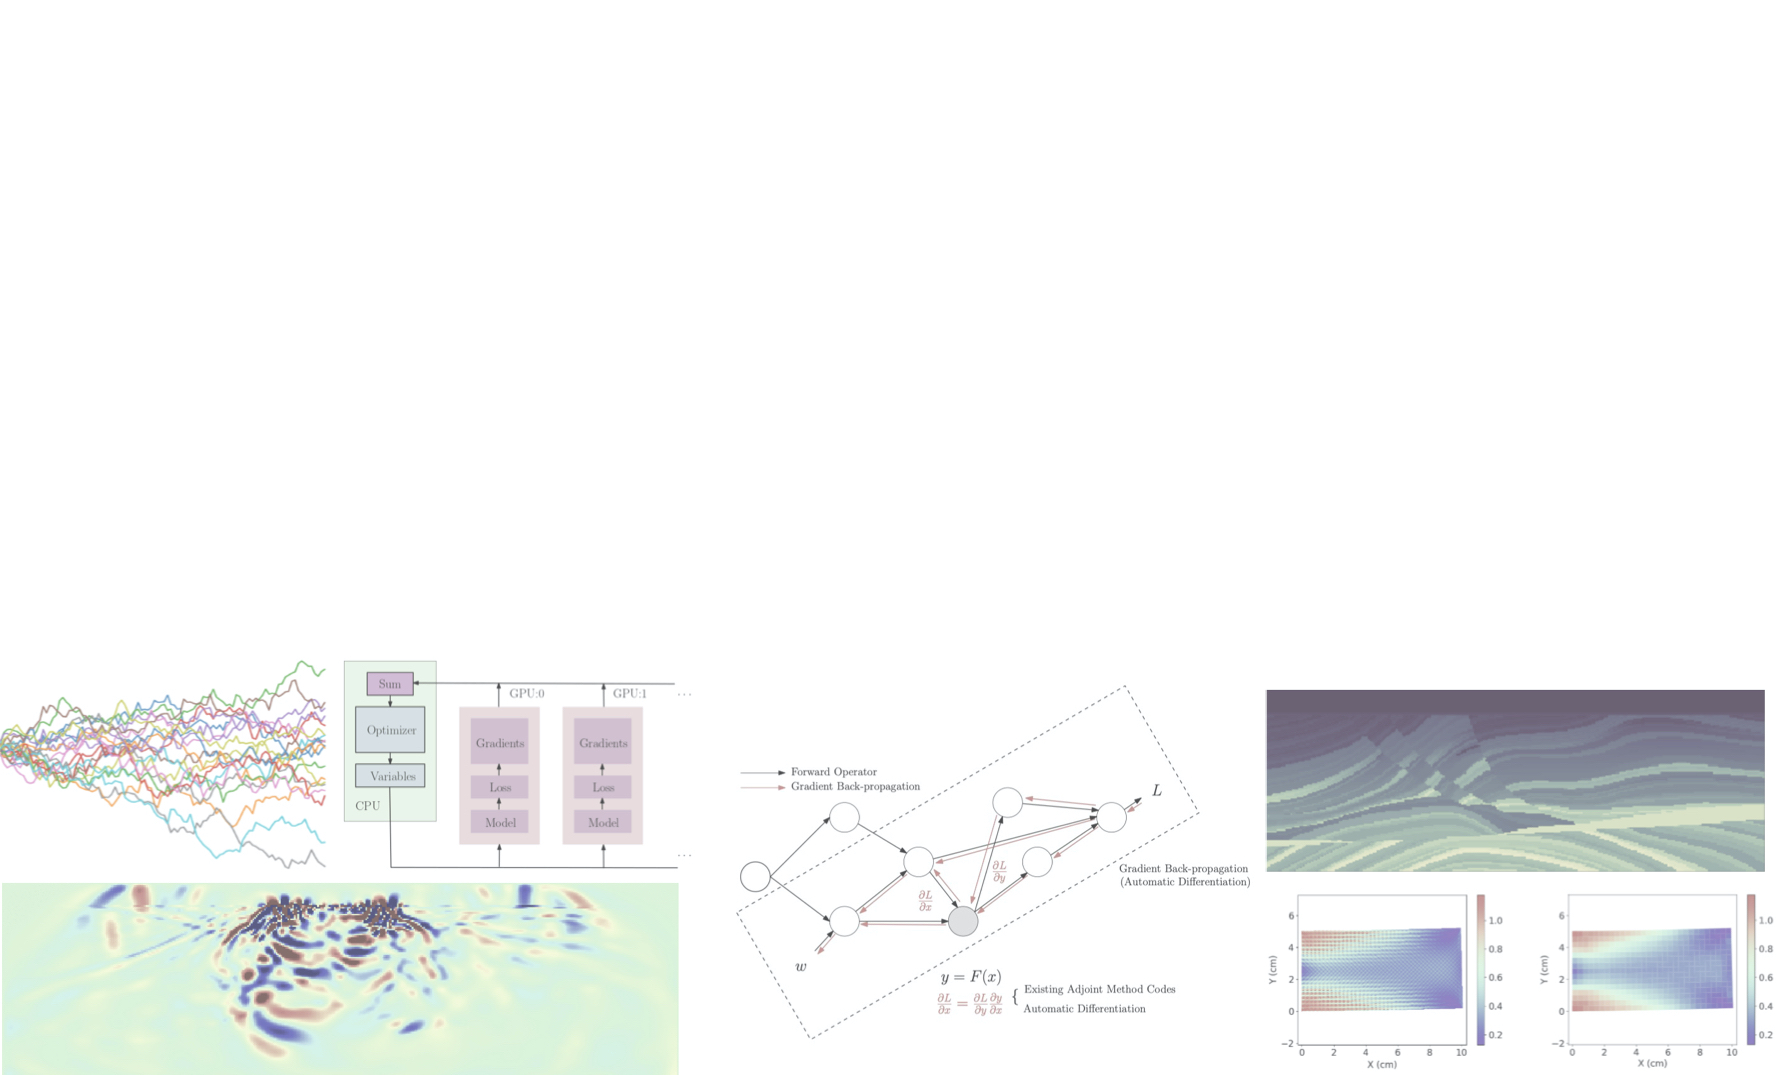
\includegraphics[width=1.0\paperwidth]{../background}}}
\end{picture}
  } 
%\usebackgroundtemplate{%
%  \includegraphics[width=\paperwidth,height=\paperheight]{figures/back}} 
\begin{frame}

\titlepage % Print the title page as the first slide


%dfa
\end{frame}
\usebackgroundtemplate{}

\section{Inverse Modeling}



\begin{frame}
	\frametitle{Inverse Modeling}
	\begin{itemize}
		\item \textbf{Inverse modeling} identifies a certain set of parameters or functions with which the outputs of the forward analysis matches the desired result or measurement.
		\item Many real life engineering problems can be formulated as inverse modeling problems: shape optimization for improving the performance of structures, optimal control of fluid dynamic systems, etc.t
	\end{itemize}
	\begin{figure}[hbt]
	\centering
  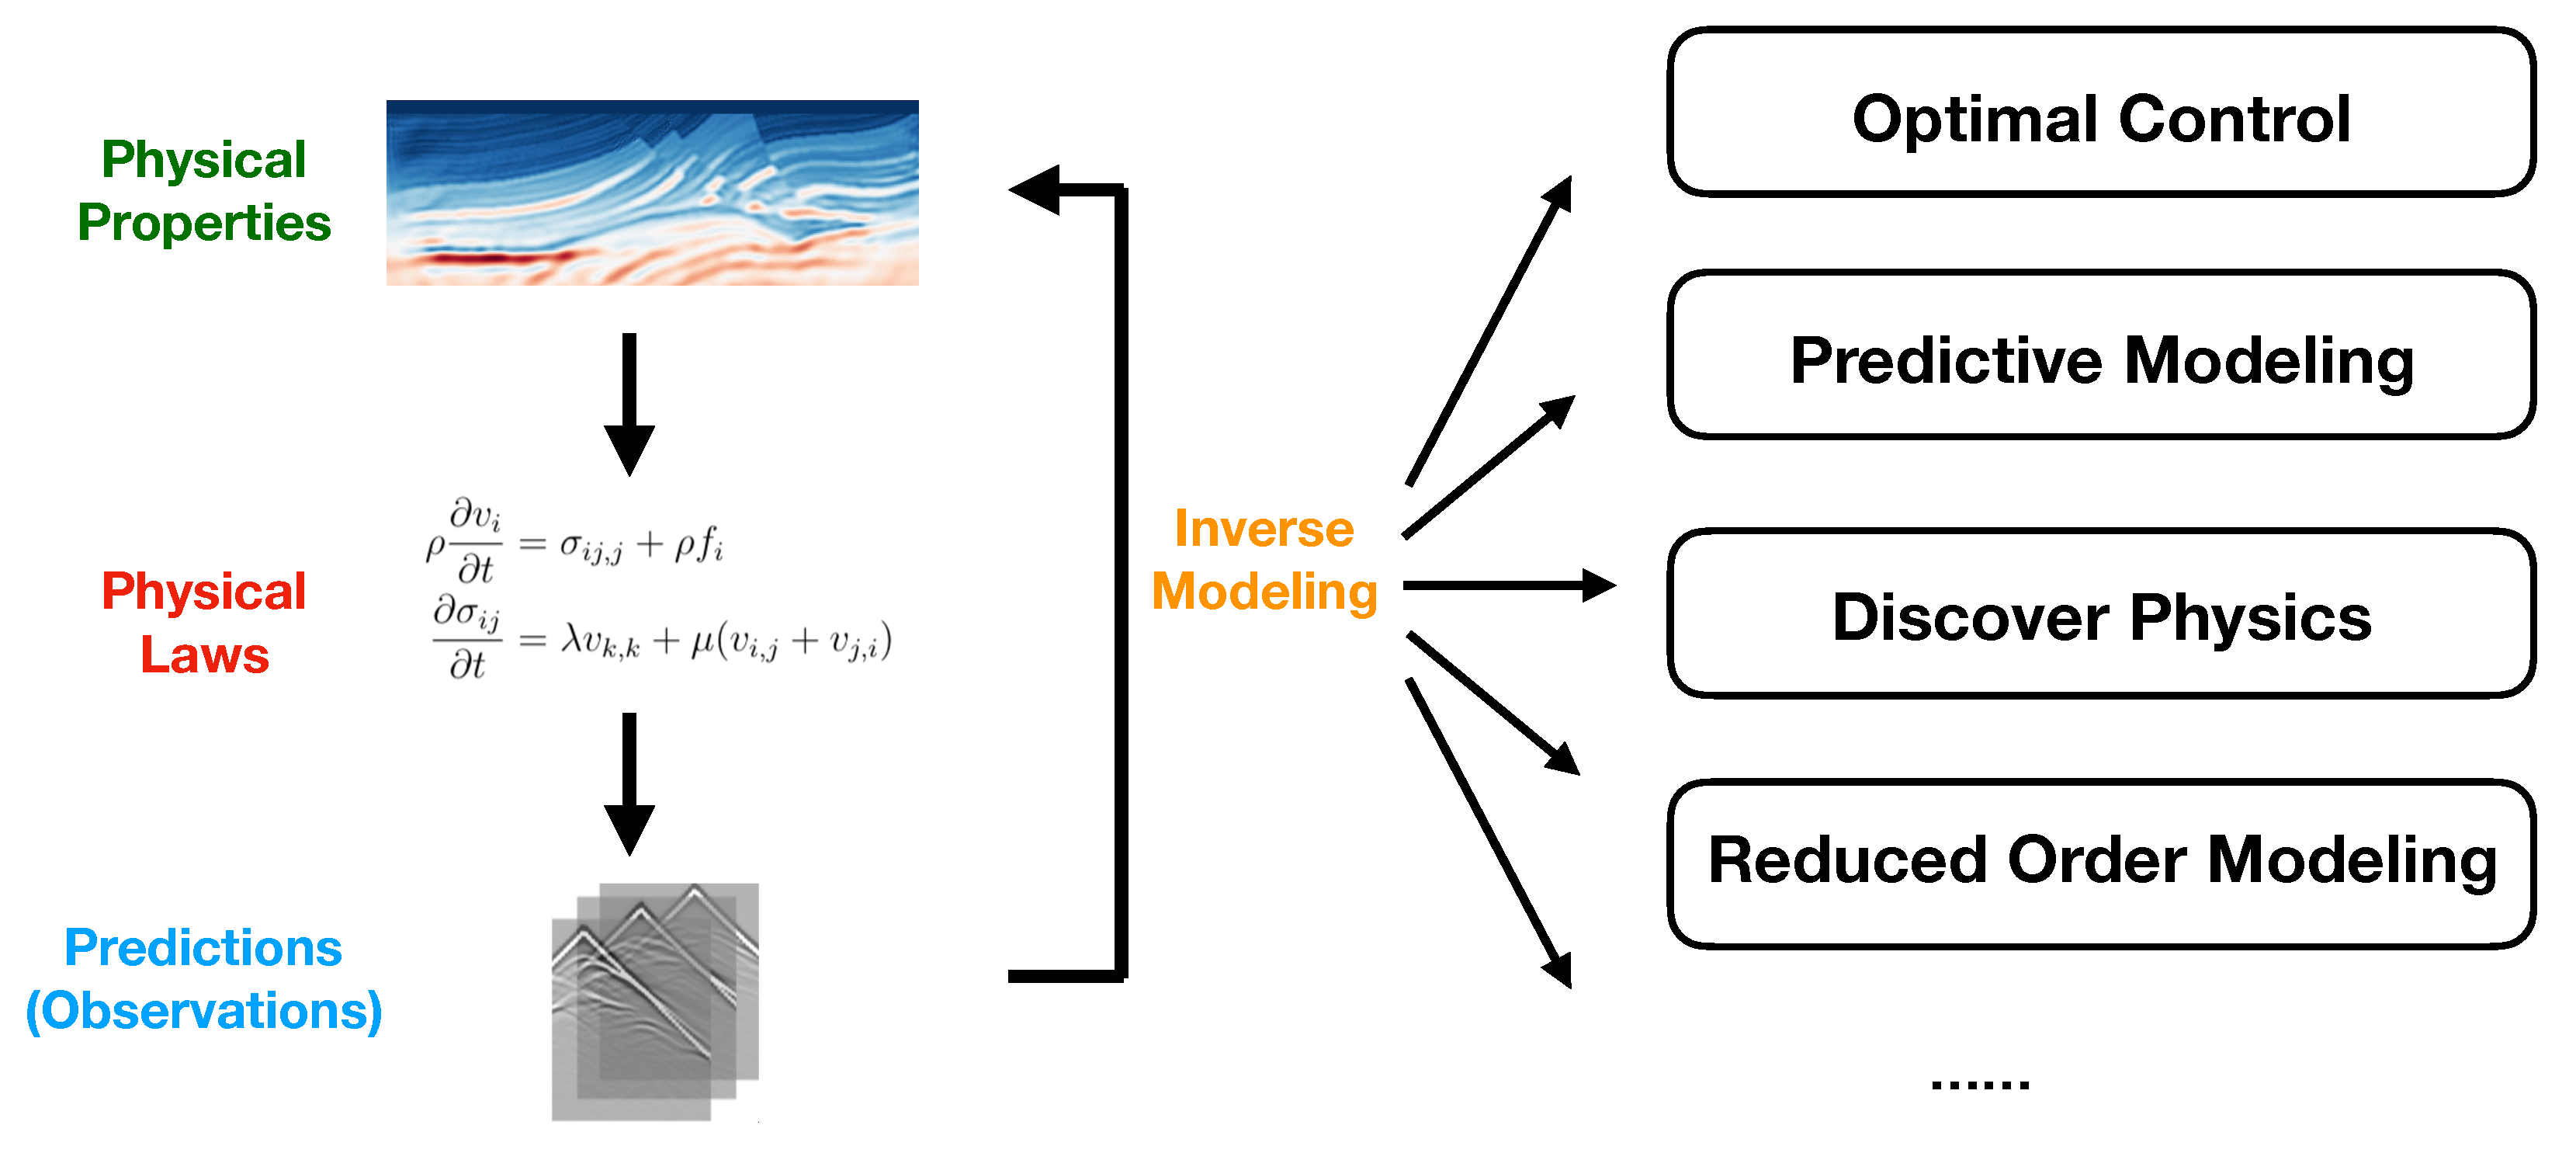
\includegraphics[width=0.8\textwidth]{../inverse2}
\end{figure}
\end{frame}

\begin{frame}
	\frametitle{Inverse Modeling}
	\begin{figure}
	\centering
  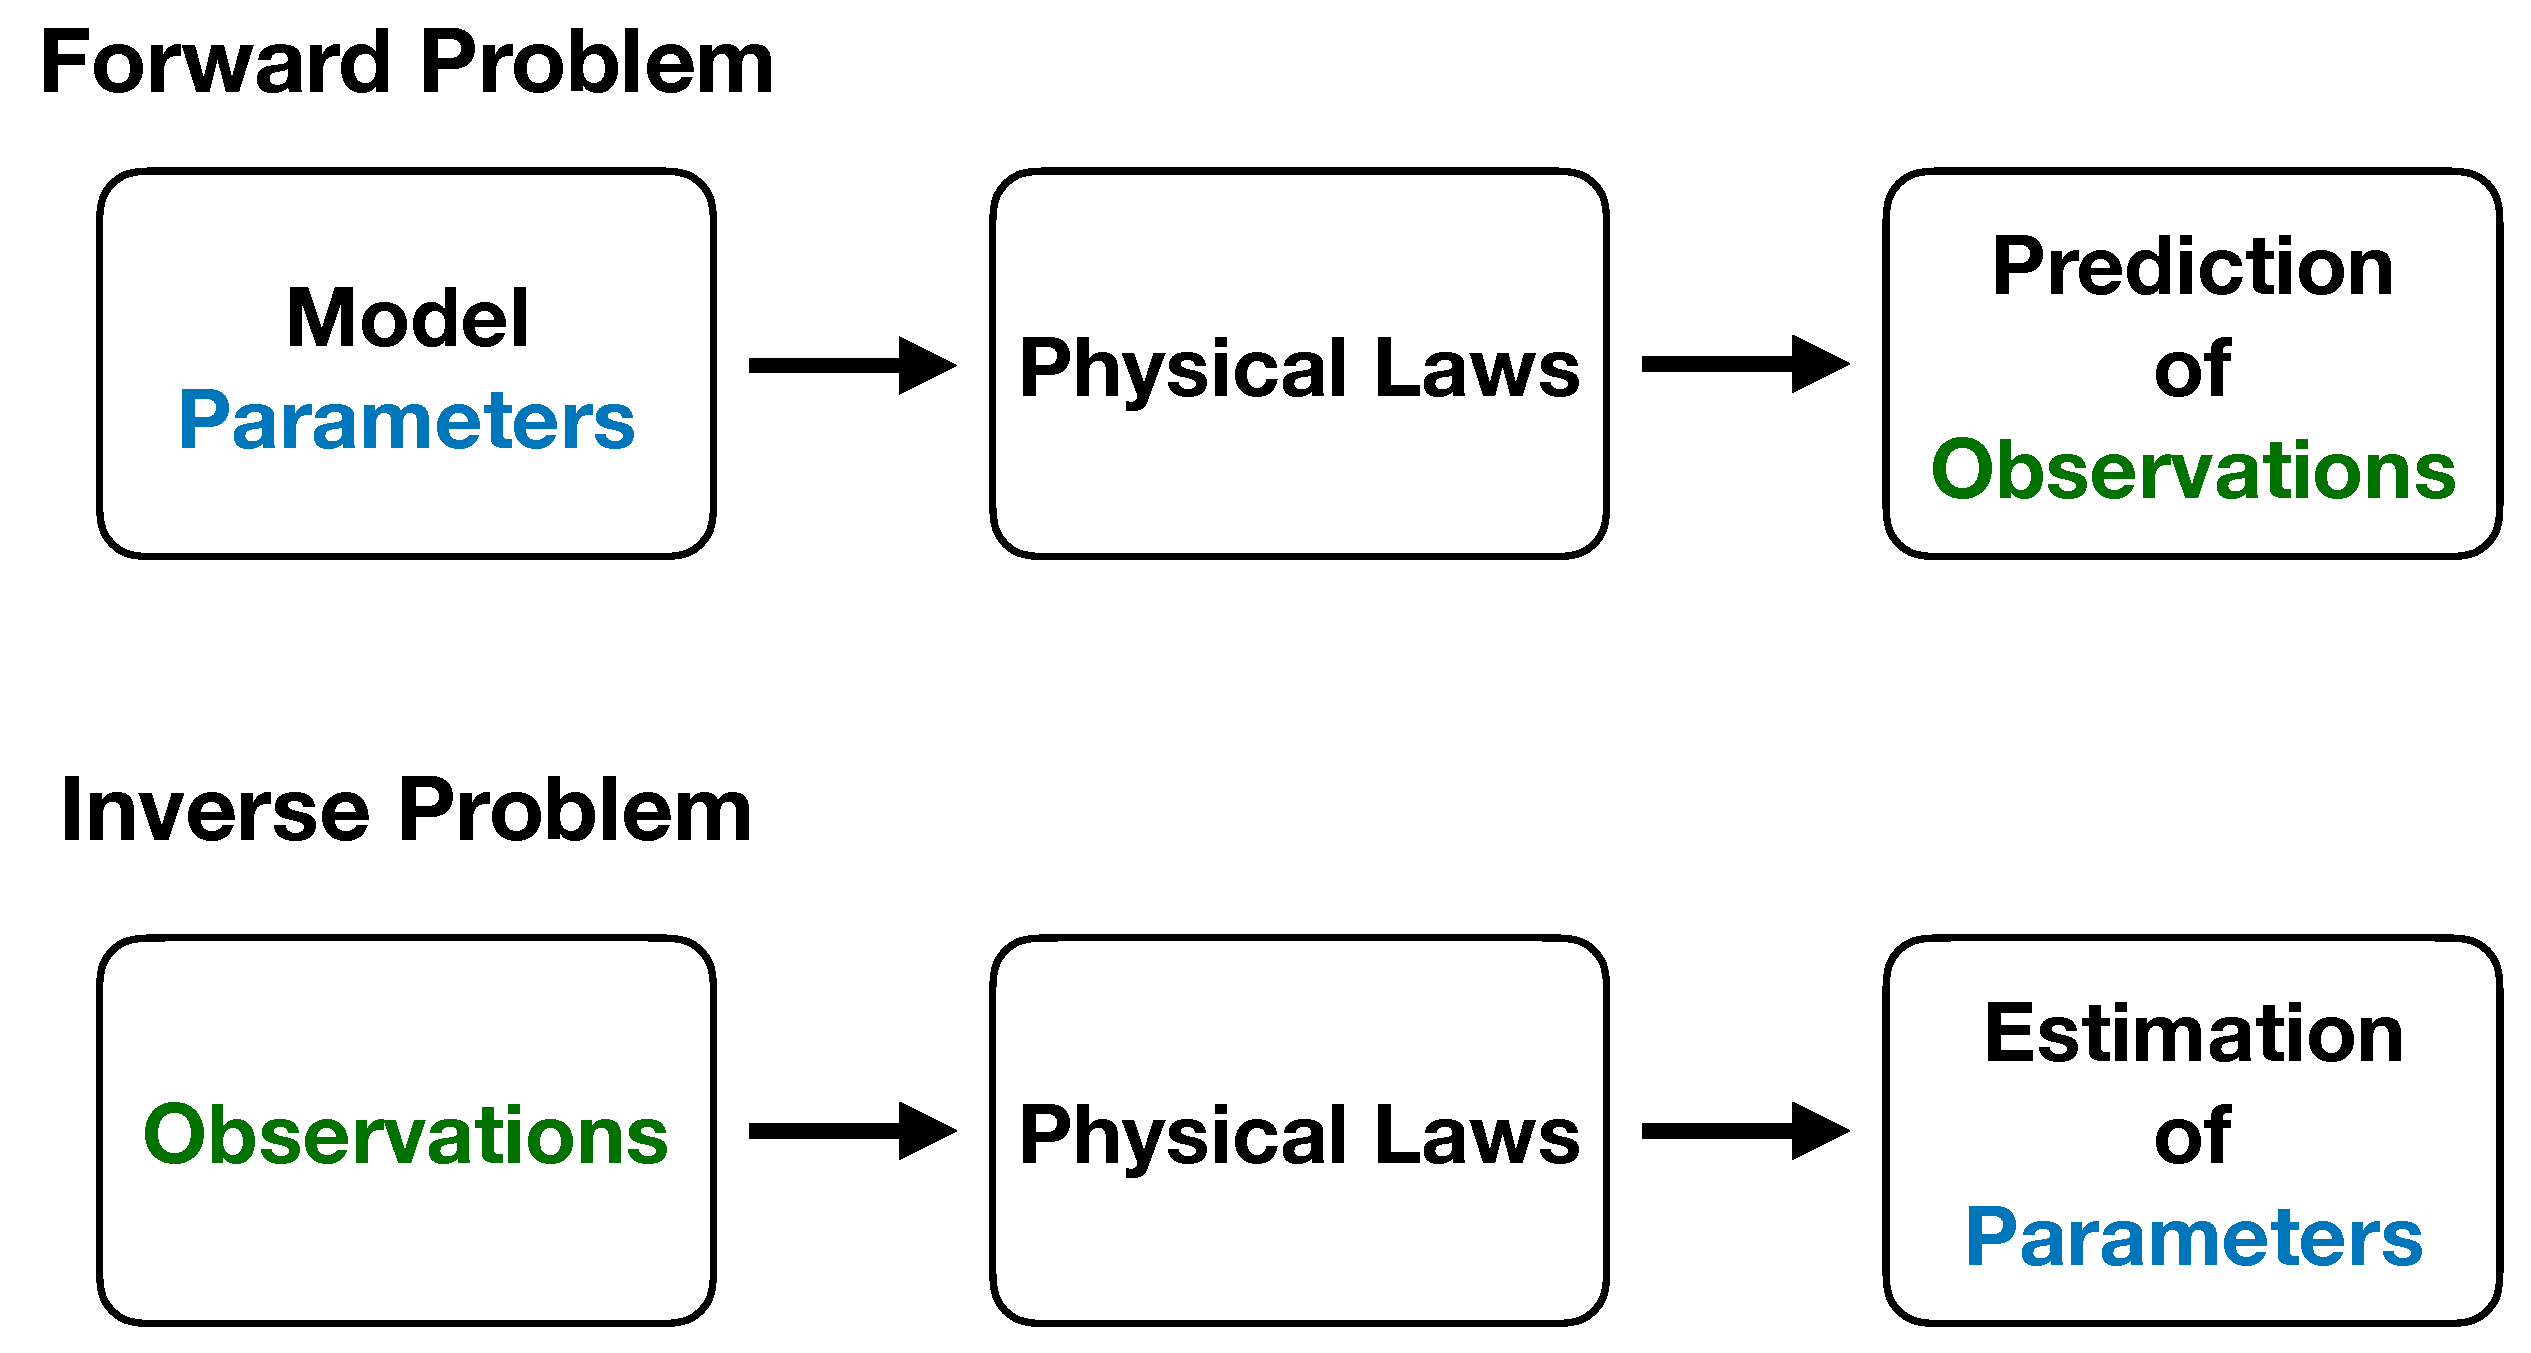
\includegraphics[width=1.0\textwidth]{../inverse3}
\end{figure}
\end{frame}

\begin{frame}
	\frametitle{Inverse Modeling for Subsurface Properties}
	 
	 There are many forms of subsurface inverse modeling problems.
	 
	 	\begin{figure}
	 	\centering
	 	\includegraphics[width=0.9\textwidth]{../inverse_types}
	 \end{figure}

\begin{center}
	\textbf{\underline{The Central Challenge}}
\end{center}	 
	\begin{center}
\textcolor{red}{\textbf{Can we have a general approach for solving these inverse problems?}}
\end{center}

\end{frame}

\begin{frame}
	\frametitle{Parameter Inverse Problem}
	We can formulate inverse modeling as a PDE-constrained optimization problem 
	\begin{equation*}
		\min_{\theta} L_h(u_h) \quad \mathrm{s.t.}\; F_h(\theta, u_h) = 0
	\end{equation*}
	\begin{itemize}
		\item The \textcolor{red}{loss function} $L_h$ measures the discrepancy between the prediction $u_h$ and the observation $u_{\mathrm{obs}}$, e.g., $L_h(u_h) = \|u_h - u_{\mathrm{obs}}\|_2^2$. 
		\item $\theta$ is the \textcolor{red}{model parameter} to be calibrated. 
		\item The \textcolor{red}{physics constraints} $F_h(\theta, u_h)=0$ are described by a system of partial differential equations. Solving for $u_h$ may require solving linear systems or applying an iterative algorithm such as the Newton-Raphson method. 
	\end{itemize}
\end{frame}




\begin{frame}
	\frametitle{Function Inverse Problem}
	
	\begin{equation*}
		\min_{\textcolor{red}{f}} L_h(u_h) \quad \mathrm{s.t.}\; F_h(\textcolor{red}{f}, u_h) = 0
	\end{equation*}
	
	What if the unknown is a \textcolor{red}{function} instead of a set of parameters?
\begin{itemize}
	\item Koopman operator in dynamical systems.
	\item Constitutive relations in solid mechanics. 
	\item Turbulent closure relations in fluid mechanics.
	\item Neural-network-based physical properties.
	\item ...
\end{itemize}

The candidate solution space is \textcolor{red}{infinite dimensional}.


	\begin{figure}[hbt]
	\includegraphics[width=0.75\textwidth]{../nnfwi.png}
\end{figure}
\end{frame}

\begin{frame}
	\frametitle{Physics Based Machine Learning}
	$$\min_{\theta} L_h(u_h) \quad \mathrm{s.t.}\;F_h(\textcolor{red}{NN_\theta}, u_h) = 0$$
	\vspace{-0.5cm}
	\begin{itemize}
		\item Deep neural networks exhibit capability of approximating high dimensional and complicated functions. 
		\item \textbf{Physics based machine learning}: \textcolor{red}{the unknown function is approximated by a deep neural network, and the physical constraints are enforced by numerical schemes}.
		\item \textcolor{red}{Satisfy the physics to the largest extent}.
	\end{itemize}
	\begin{figure}[hbt]
  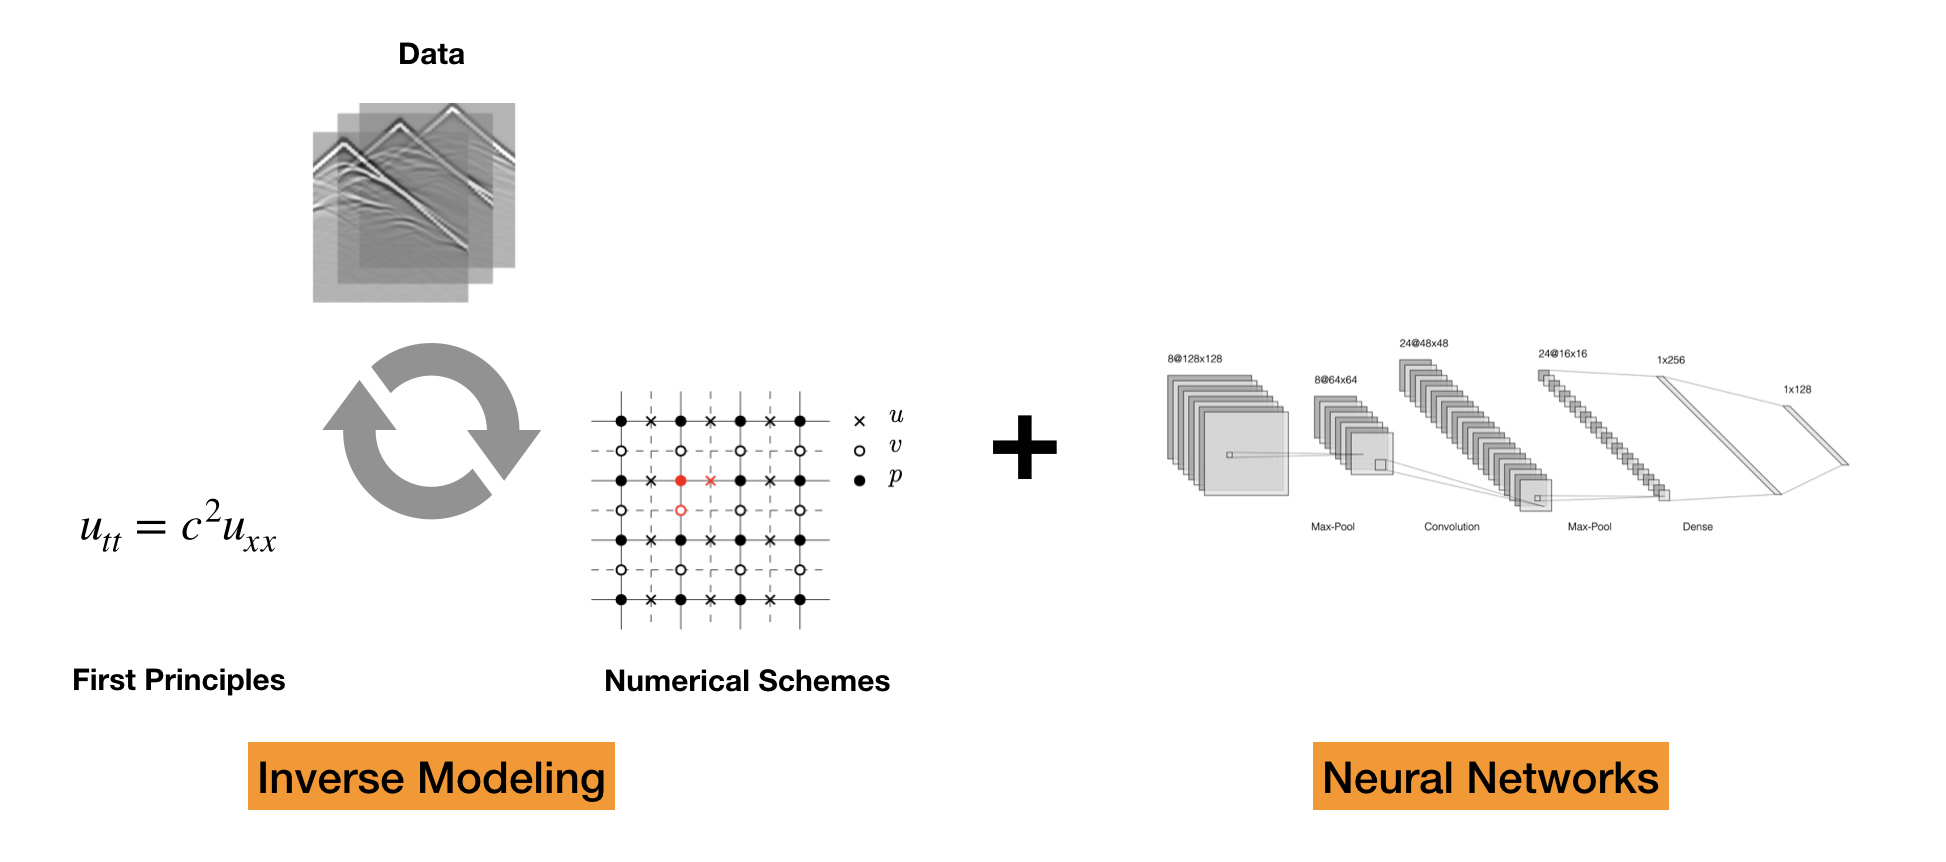
\includegraphics[width=0.75\textwidth]{../physics_based_machine_learning.png}
\end{figure}
\end{frame}



\begin{frame}
	\frametitle{Gradient Based Optimization}
	\begin{equation}\label{equ:opt}
		\min_{\theta} L_h(u_h) \quad \mathrm{s.t.}\; F_h(\theta, u_h) = 0
		\end{equation}
	
	\begin{itemize}
		\item We can now apply a gradient-based optimization method to (\ref{equ:opt}).
		\item The key is to \textcolor{red}{calculate the gradient descent direction} $g^k$
		$$\theta^{k+1} \gets \theta^k - \alpha g^k$$ 
	\end{itemize}
	
	\begin{figure}[hbt]
	\centering
  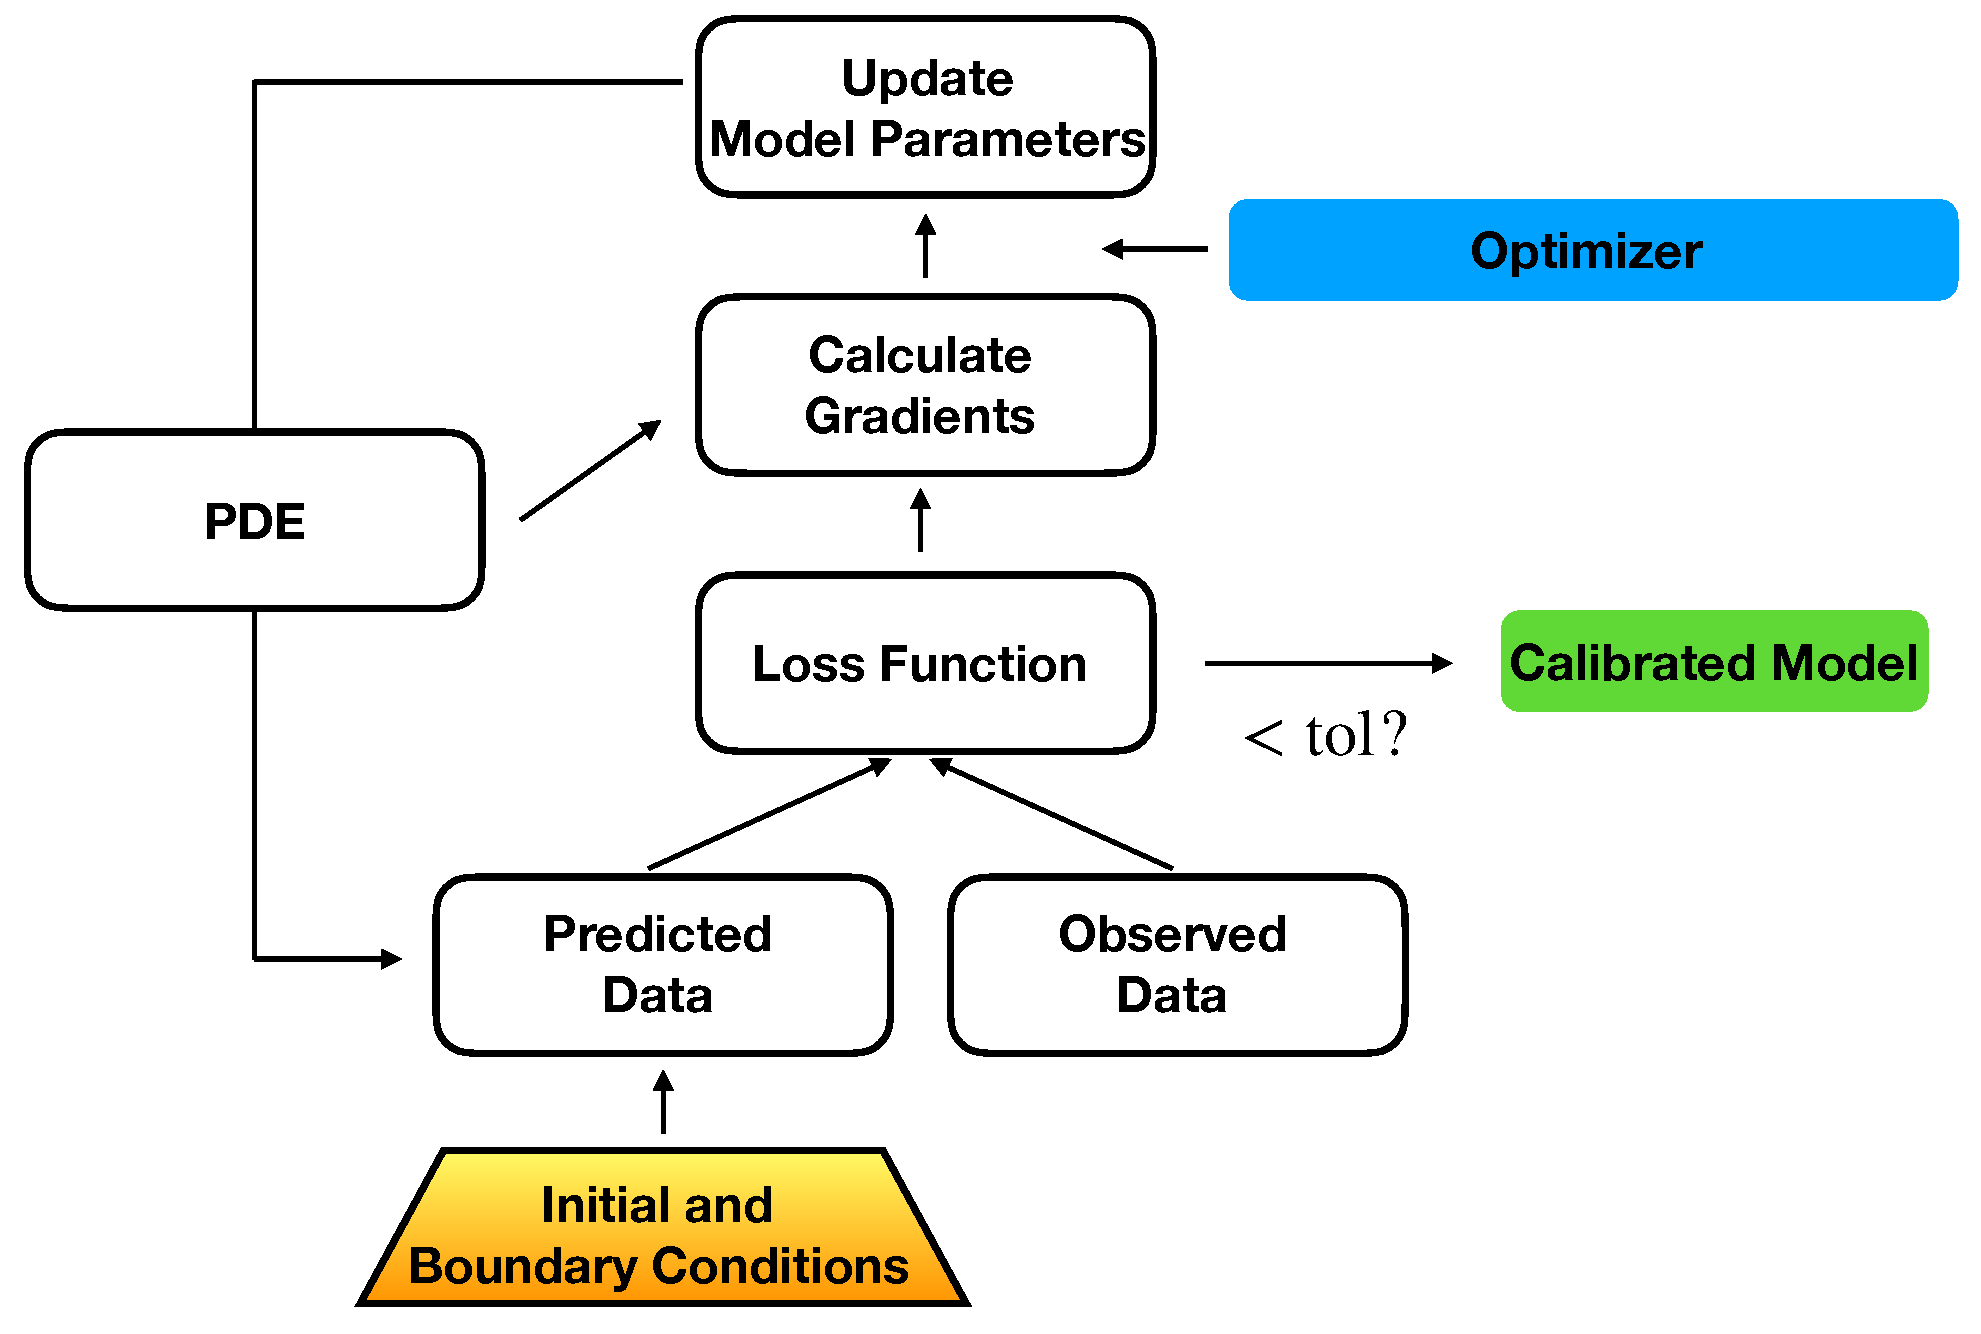
\includegraphics[width=0.6\textwidth]{../im.pdf}
\end{figure}

\end{frame}



\section{Automatic Differentiation}

\begin{frame}
	\frametitle{Automatic Differentiation}
The fact that bridges the \textcolor{red}{technical} gap between machine learning and inverse modeling:
	\begin{itemize}
		\item Deep learning (and many other machine learning techniques) and numerical schemes share the same computational model: composition of individual operators. 
	\end{itemize}
	

\begin{minipage}[b]{0.4\textwidth}




\begin{center}
\textcolor{red}{Mathematical Fact}

\

	Back-propagation 

$||$

Reverse-mode

 Automatic Differentiation 

$||$
 
 Discrete 
 
 Adjoint-State Method
\end{center}
\end{minipage}~
\begin{minipage}[b]{0.6\textwidth}
\begin{figure}[hbt]
\centering
  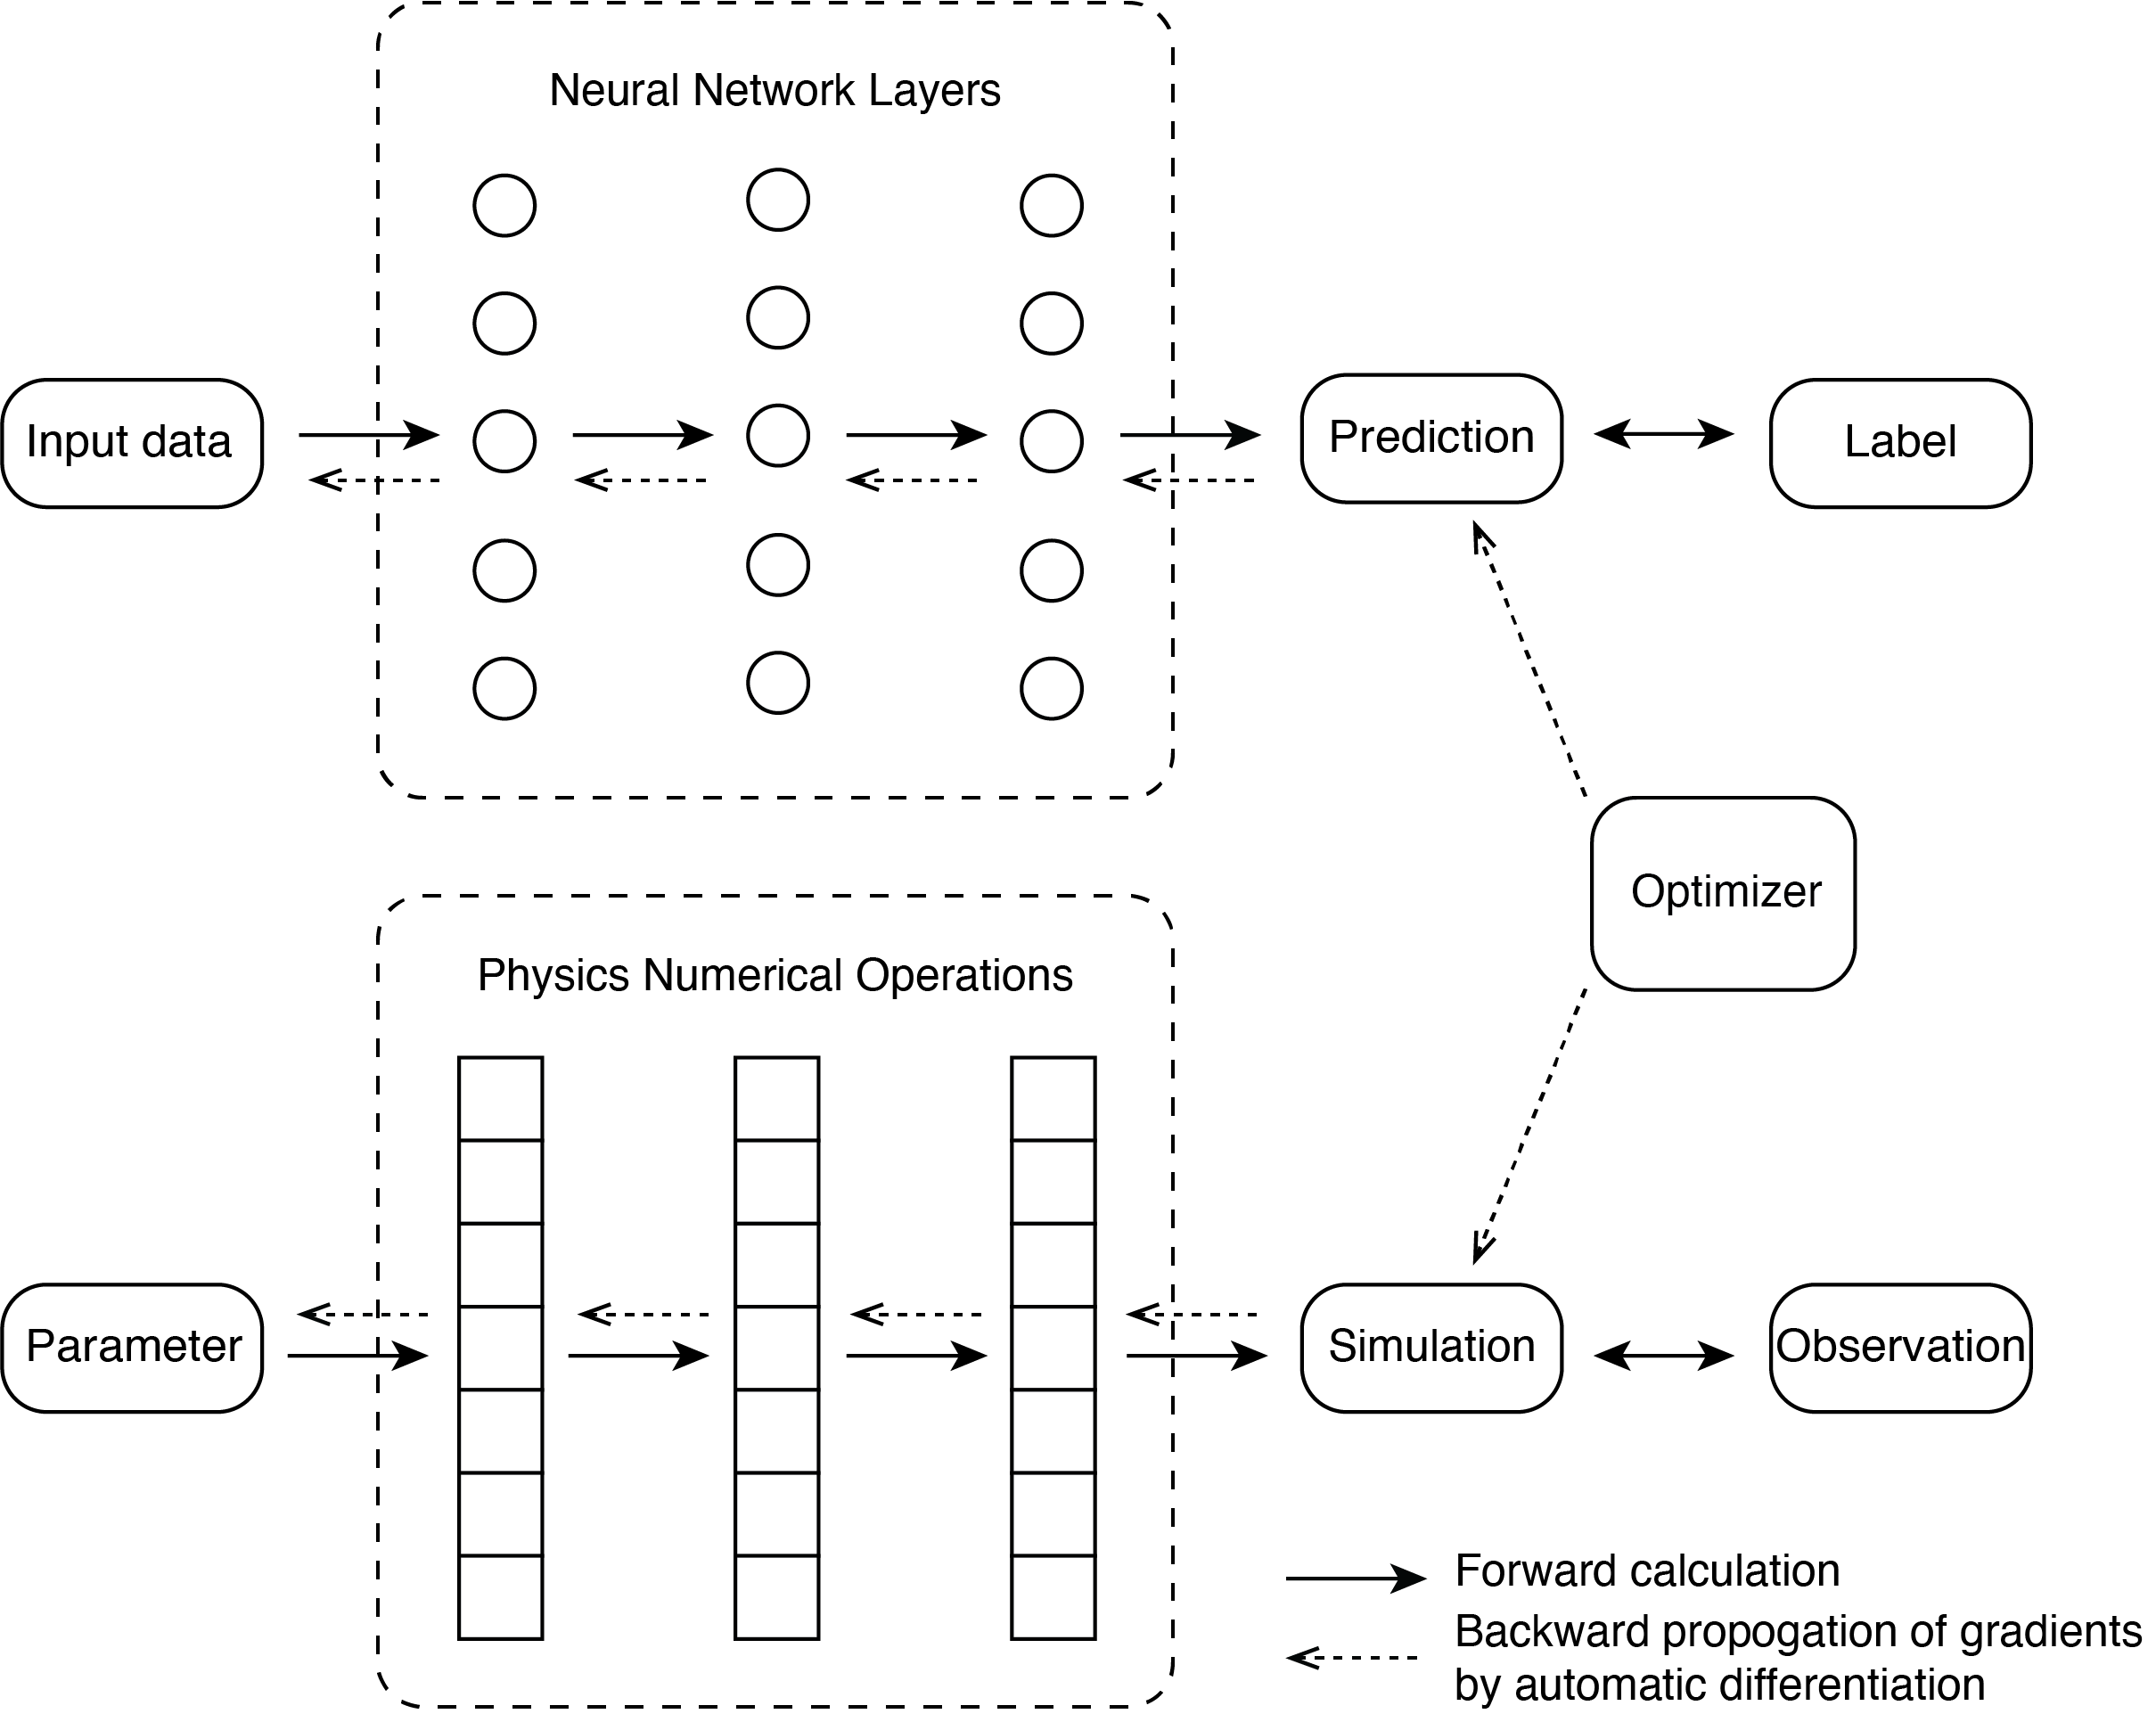
\includegraphics[width=0.8\textwidth]{../compare-NN-PDE.png}
\end{figure}
\end{minipage}

\end{frame}




\begin{frame}
	\frametitle{Forward Mode vs. Reverse Mode}
	
	\begin{itemize}
		\item Reverse mode automatic differentiation evaluates gradients in the \textcolor{red}{reverse order} of forward computation. 
		\item Reverse mode automatic differentiation is a more efficient way to compute gradients of a many-to-one mapping $J(\alpha_1, \alpha_2, \alpha_3,\alpha_4)$ $\Rightarrow$ suitable for minimizing a loss (misfit) function. 
	\end{itemize}
	
	\begin{figure}[hbt]
		\includegraphics[width=0.8\textwidth]{../fdrd}
	\end{figure}
	
	
	
\end{frame}


\begin{frame}
	\frametitle{Computational Graph for Numerical Schemes}
	
	\begin{itemize}
		\item To leverage automatic differentiation for inverse modeling, we need to express the numerical schemes in the ``AD language'': computational graph. 
		\item No matter how complicated a numerical scheme is, it can be decomposed into a collection of operators that are interlinked via state variable dependencies. 
	\end{itemize}
	
	\begin{figure}[hbt]
  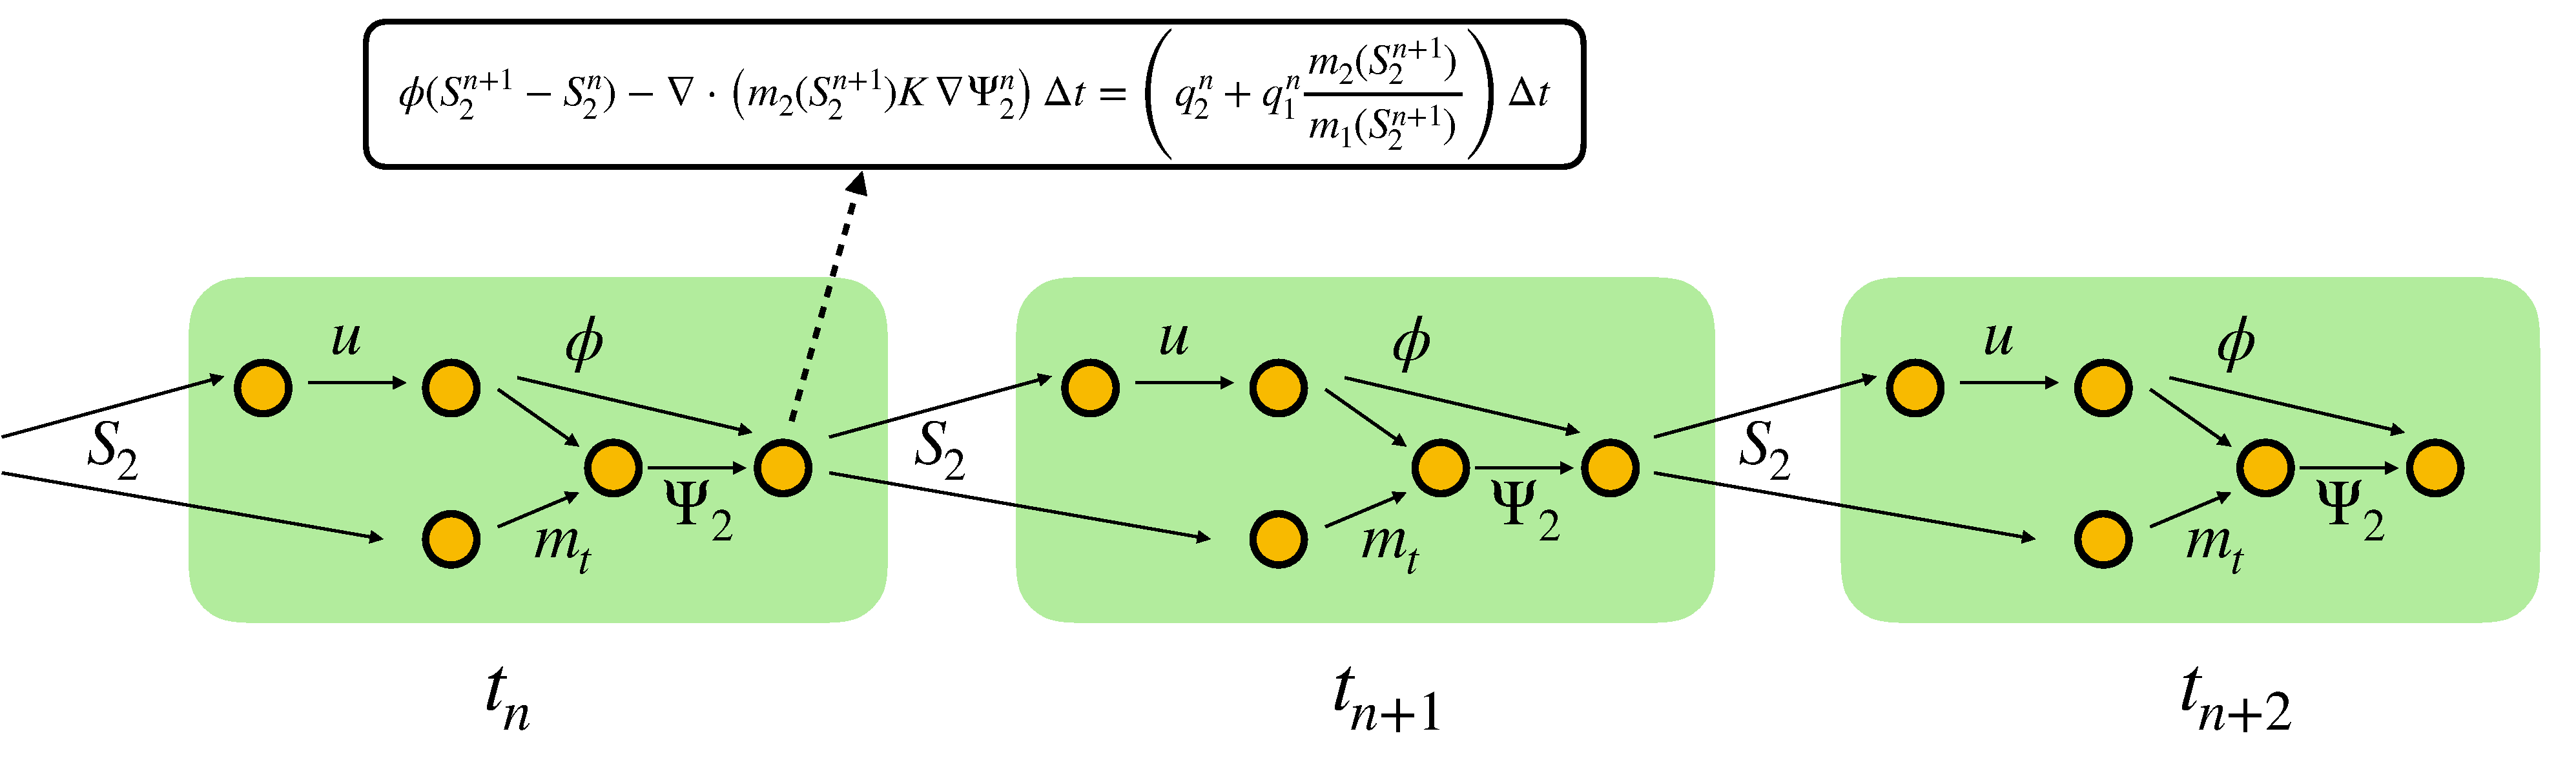
\includegraphics[width=1.0\textwidth]{../cgnum}
\end{figure}

	
	
\end{frame}





%\begin{frame}
%	\frametitle{Code Example}
%	\begin{itemize}
%		\item  Find $b$ such that $u(0.5)=1.0$ and
%		$$-bu''(x)+u(x) = 8 + 4x - 4x^2, x\in[0,1], u(0)=u(1)=0$$
%	\end{itemize}
%	\begin{figure}[hbt]
%  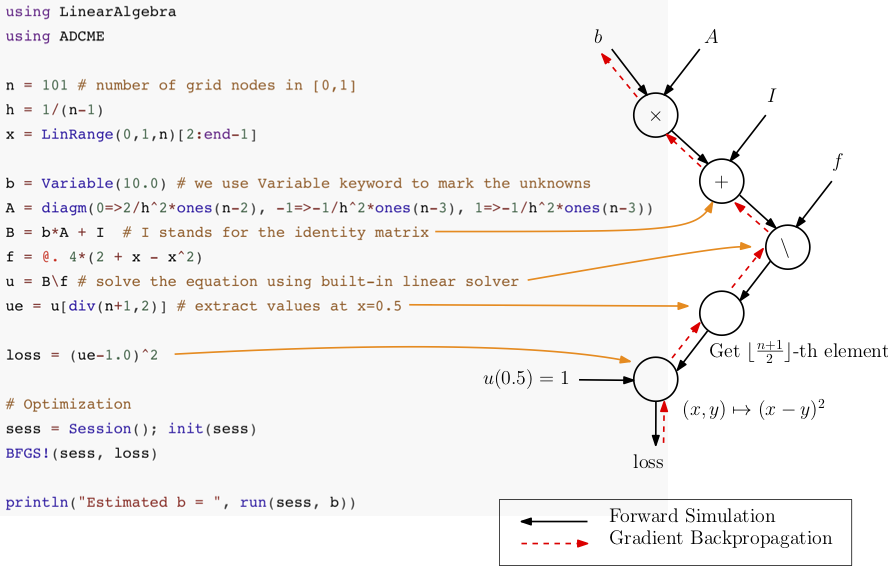
\includegraphics[width=0.8\textwidth]{../code.png}
%\end{figure}
%\end{frame}


\section{Physics Constrained Learning}
\begin{frame}


	\frametitle{Challenges in AD}
	
	
	\begin{minipage}[t]{0.49\textwidth}
	\vspace{-3cm}
\begin{itemize}
	\item Most AD frameworks only deal with \textcolor{red}{explicit operators}, i.e., the functions that has analytical derivatives that are easy to implement.  
	\item Many scientific computing algorithms are \textcolor{red}{iterative} or \textcolor{red}{implicit} in nature.
\end{itemize}
\end{minipage}~
\begin{minipage}[t]{0.49\textwidth}
  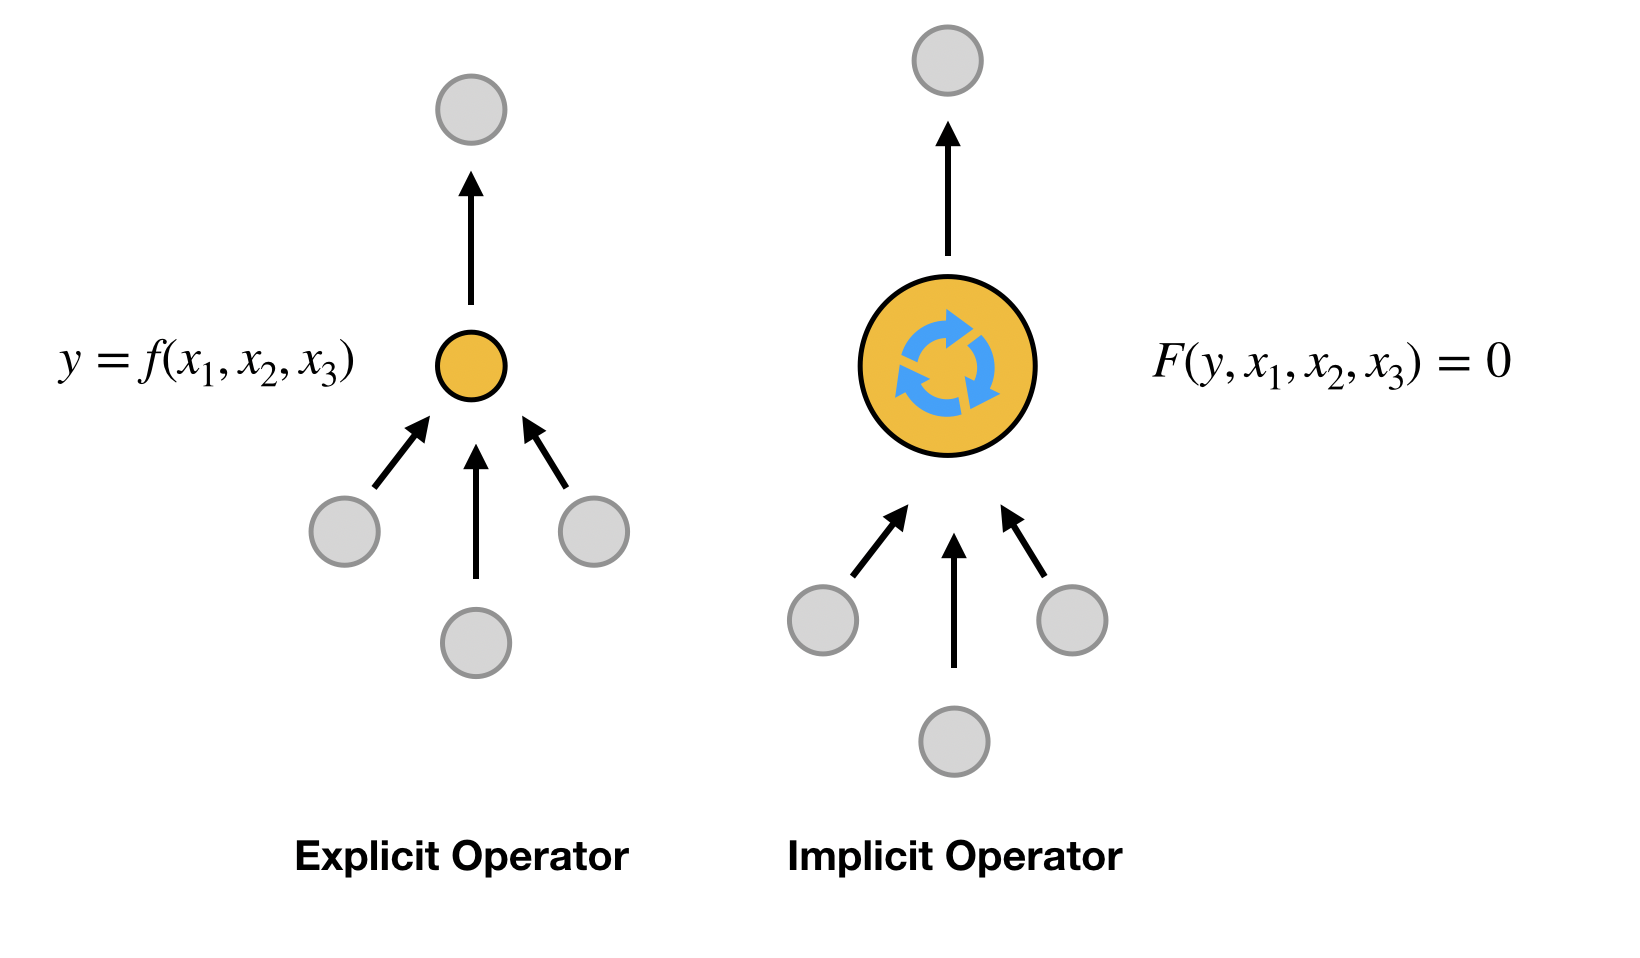
\includegraphics[width=1.0\textwidth]{../sim.png}
\end{minipage}

	% Please add the following required packages to your document preamble:
% \usepackage{booktabs}
\begin{table}[]
\begin{tabular}{@{}lll@{}}
\toprule
Linear/Nonlinear & Explicit/Implicit & Expression   \\ \midrule
Linear           & Explicit          & $y=Ax$       \\
Nonlinear        & Explicit          & $y = F(x)$   \\
\textbf{Linear}           & \textbf{Implicit}          & $Ay = x$     \\
\textbf{Nonlinear}        & \textbf{Implicit}          & $F(x,y) = 0$ \\ \bottomrule
\end{tabular}
\end{table}
\end{frame}



\begin{frame}
	\frametitle{Implicit Operators in Subsurface Modeling}
		
		\begin{itemize}
			\item For reasons such as nonlinearity and stability, implicit operators (schemes) are almost everywhere in subsurface modeling...
				\begin{figure}
				\centering
				\includegraphics[width=0.9\textwidth]{../nonlinear.PNG}
			\end{figure}
			\item The ultimate solution: \textcolor{red}{design ``differentiable'' implicit operators}.
		\end{itemize}
		
\end{frame}

\begin{frame}
	\frametitle{Example}
	
\begin{itemize}
	\item Consider a function $f:x\rightarrow y$, which is implicitly defined by 
	$$F(x,y) = x^3 - (y^3+y) = 0$$
If not using the cubic formula for finding the roots, the forward computation consists of iterative algorithms, such as the Newton's method and bisection method
\end{itemize}



\begin{minipage}[t]{0.48\textwidth}
\centering
\begin{algorithmic}
\State $y^0 \gets 0$
\State $k \gets 0$
\While {$|F(x, y^k)|>\epsilon$}
\State $\delta^k \gets F(x, y^k)/F'_y(x,y^k)$
\State $y^{k+1}\gets y^k - \delta^k$
\State $k \gets k+1$
\EndWhile
\State \textbf{Return} $y^k$
\end{algorithmic}
\end{minipage}~
\begin{minipage}[t]{0.48\textwidth}
\centering
\begin{algorithmic}
\State $l \gets -M$, $r\gets M$, $m\gets 0$
\While {$|F(x, m)|>\epsilon$}
\State $c \gets \frac{a+b}{2}$
\If{$F(x, m)>0$}
\State $a\gets m$
\Else
\State $b\gets m$
\EndIf
\EndWhile
\State \textbf{Return} $c$
\end{algorithmic}

\end{minipage}	

\end{frame}


\begin{frame}
	\frametitle{Example}
	
	\begin{itemize}
%		\item A simple approach is to save part or all intermediate steps, and ``back-propagate''. This approach is expensive in both computation and memory\footnote{Ablin, Pierre, Gabriel Peyré, and Thomas Moreau. ``Super-efficiency of automatic differentiation for functions defined as a minimum.''}.
%		\item Nevertheless, the simple approach works in some scenarios where accuracy or cost is not an issue, e.g., automatic differetiation of soft-DTW and Sinkhorn distance. 
		\item An efficient way is to apply the \textcolor{red}{implicit function theorem}. For our example, $F(x,y)=x^3-(y^3+y)=0$, treat $y$ as a function of $x$ and take the derivative on both sides
		$$3x^2 - 3y(x)^2y'(x)-1=0\Rightarrow y'(x) = \frac{3x^2-1}{3y(x)^2}$$
	The above gradient is \textcolor{red}{exact}.
	\end{itemize}
	\begin{center}
			\textbf{Can we apply the same idea to inverse modeling?}
	\end{center}

\end{frame}


\begin{frame}
	\frametitle{Physics Constrained Learning}
	$${\small    \min_{\theta}\; L_h(u_h) \quad \mathrm{s.t.}\;\; F_h(\theta, u_h) = 0}$$
	\begin{itemize}
		\item Assume that we solve for $u_h=G_h(\theta)$ with $F_h(\theta, u_h)=0$, and then
		      $${\small\tilde L_h(\theta)  = L_h(G_h(\theta))}$$
		\item Applying the \textcolor{red}{implicit function theorem}
		      {  \scriptsize
			      \begin{equation*}
				      \frac{{\partial {F_h(\theta, u_h)}}}{{\partial \theta }} + {\frac{{\partial {F_h(\theta, u_h)}}}{{\partial {u_h}}}}
				      \textcolor{red}{\frac{\partial G_h(\theta)}{\partial \theta}}
				      = 0 \Rightarrow
				      \textcolor{red}{\frac{\partial G_h(\theta)}{\partial \theta}} =  -\Big( \frac{{\partial {F_h(\theta, u_h)}}}{{\partial {u_h}}} \Big)^{ - 1} \frac{{\partial {F_h(\theta, u_h)}}}{{\partial \theta }}
			      \end{equation*}
		      }
		\item Finally we have
			      {\scriptsize
				      \begin{equation*}
					      \boxed{\frac{{\partial {{\tilde L}_h}(\theta )}}{{\partial \theta }}
					      = \frac{\partial {{ L}_h}(u_h )}{\partial u_h}\frac{\partial G_h(\theta)}{\partial \theta}=
					      - \textcolor{red}{ \frac{{\partial {L_h}({u_h})}}{{\partial {u_h}}} } \;
					      \textcolor{blue}{ \Big( {\frac{{\partial {F_h(\theta, u_h)}}}{{\partial {u_h}}}\Big|_{u_h = {G_h}(\theta )}} \Big)^{ - 1} } \;
					      \textcolor{ForestGreen}{ \frac{{\partial {F_h(\theta, u_h)}}}{{\partial \theta }}\Big|_{u_h = {G_h}(\theta )} }
					      }
				      \end{equation*}
			      }

	\end{itemize}

\end{frame}



\section{Applications}


\begin{frame}
	\frametitle{Parameter Inverse Problem: Elastic Full Waveform Inversion for Subsurface Flow Problems}
	\begin{figure}[hbt]
  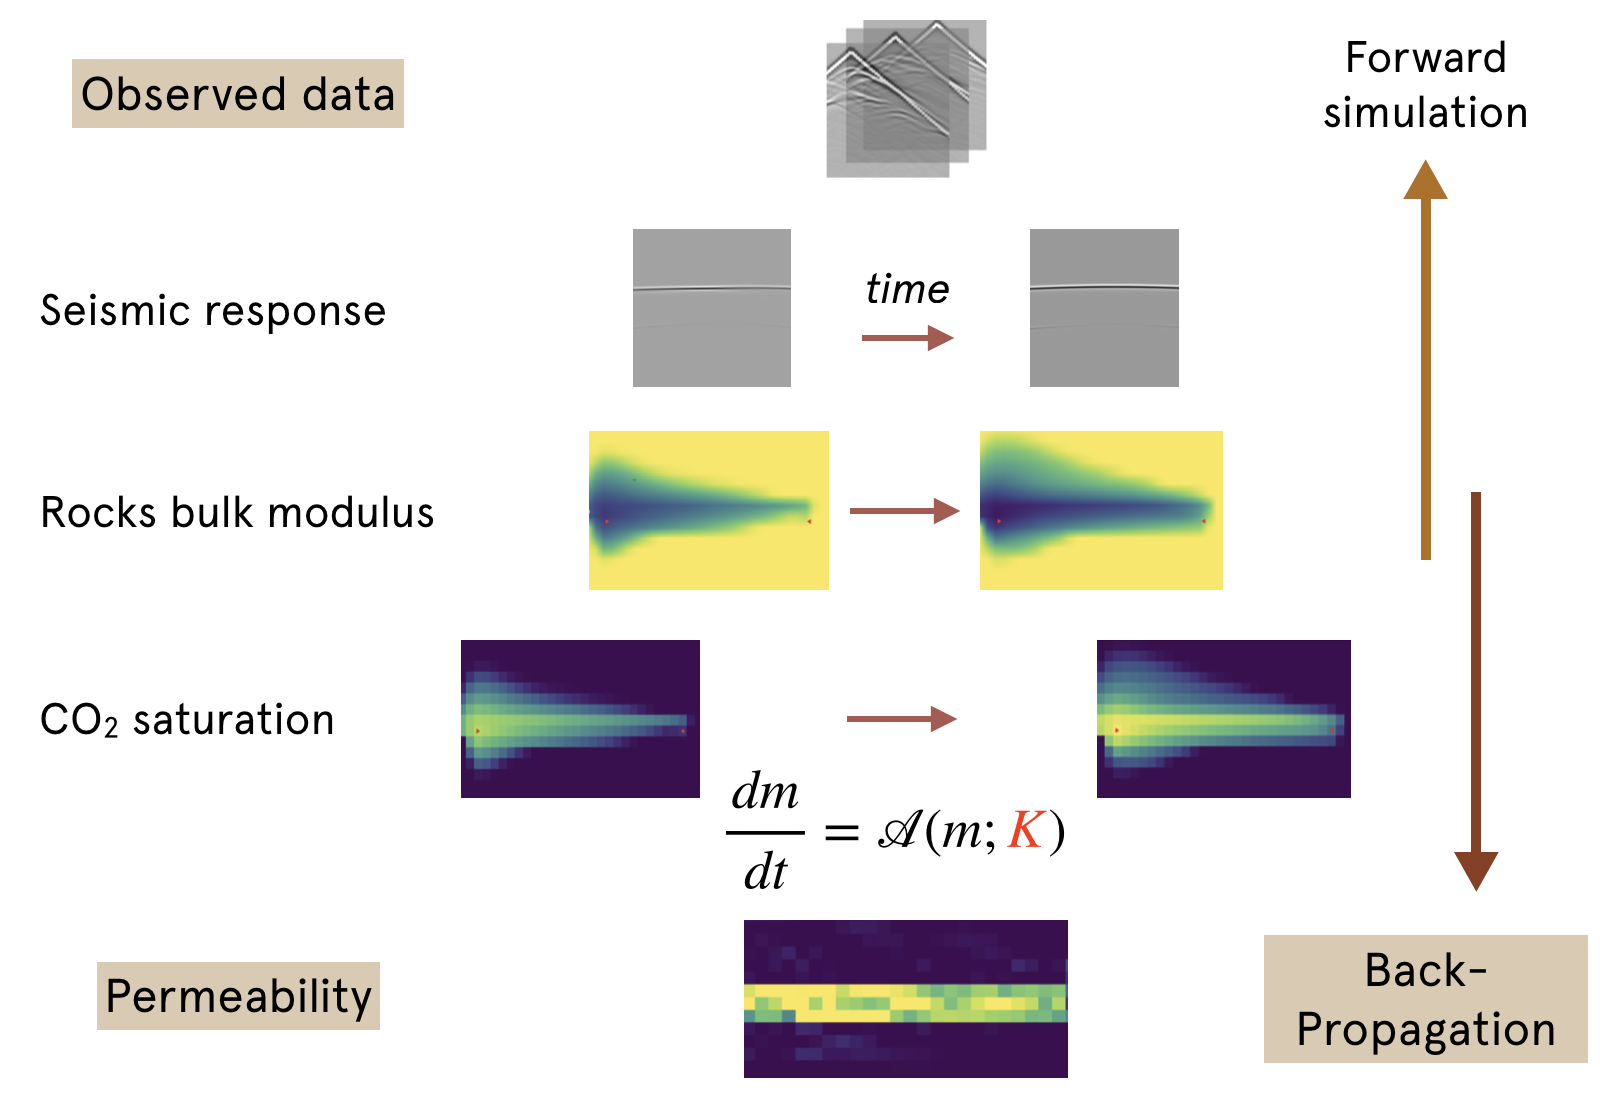
\includegraphics[width=0.8\textwidth]{../geo.png}
\end{figure}
\end{frame}

\begin{frame}
\frametitle{Fully Nonlinear Implicit Schemes}
\begin{itemize}
	\item The governing equation is a nonlinear PDE
\begin{minipage}[b]{0.48\textwidth}
{\scriptsize
	\begin{align*}
	&\frac{\partial }{{\partial t}}(\phi {{S_i}}{\rho _i}) + \nabla  \cdot ({\rho _i}{\mathbf{v}_i}) = {\rho _i}{q_i},\quad 
      i = 1,2	\\
     & S_{1} + S_{2} = 1\\
      &{\mathbf{v}_i} = - \frac{{\textcolor{blue}{K}{\textcolor{red}{k_{ri}}}}}{{{\tilde{\mu}_i}}}(\nabla {P_i} - g{\rho _i}\nabla Z), \quad
      i=1, 2\\
	&k_{r1}(S_1) = \frac{k_{r1}^o S_1^{L_1}}{S_1^{L_1} + E_1 S_2^{T_1}}\\
	&k_{r2}(S_1) = \frac{ S_2^{L_2}}{S_2^{L_2} + E_2 S_1^{T_2}}
	\end{align*}
	}
\end{minipage}~\vline
\begin{minipage}[b]{0.48\textwidth}
\flushleft
	{\scriptsize \begin{eqnarray*}
 && \rho \frac{\partial v_z}{\partial t} = \frac{\partial \sigma_{zz}}{\partial z} + \frac{\partial \sigma_{xz}}{\partial x} \nonumber \\
 && \rho \frac{\partial v_x}{\partial t} = \frac{\partial \sigma_{xx}}{\partial x} + \frac{\partial \sigma_{xz}}{\partial z} \nonumber \\
 && \frac{\partial \sigma_{zz}}{\partial t} = (\lambda + 2\mu)\frac{\partial v_z}{\partial z} + \lambda\frac{\partial v_x}{\partial x} \nonumber \\
 && \frac{\partial \sigma_{xx}}{\partial t} = (\lambda + 2\mu)\frac{\partial v_x}{\partial x} + \lambda\frac{\partial v_z}{\partial z} \nonumber \\
 && \frac{\partial \sigma_{xz}}{\partial t} = \mu (\frac{\partial v_z}{\partial x} + \frac{\partial v_x}{\partial z}),
\end{eqnarray*}}
\end{minipage}

	\item For stability and efficiency, implicit methods are the industrial standards. 
{\scriptsize	$$\phi (S_2^{n + 1} - S_2^n) - \nabla \cdot \left( {{m_{2}}(S_2^{n + 1})K\nabla \Psi _2^n} \right) \Delta t = 
\left(q_2^n + q_1^n \frac{m_2(S^{n+1}_2)}{m_1(S^{n+1}_2)}\right) 
\Delta t\quad m_i(s) = \frac{k_{ri}(s)}{\tilde \mu_i}
$$} 
\end{itemize}

\end{frame}

\begin{frame}
	\frametitle{Inverse Modeling Workflow}
	Traditionally, the inversion is typically solved by separately inverting the wave equation (FWI) and the flow transport equations. 
	\begin{figure}
		\centering
			\includegraphics[width=0.8\textwidth]{../coupled3}
		\includegraphics[width=0.7\textwidth]{../coupled1}
	\end{figure}
\end{frame}


\begin{frame}
	\frametitle{Coupled Inversion vs. Decoupled Inversion}
	We found that \textcolor{red}{by coupled inversion reduces the artifacts from FWI significantly and yields a substantially better results}. 
	\begin{figure}
		\centering
		\includegraphics[width=0.6\textwidth]{../coupled2}
	\end{figure}
\end{frame}

\begin{frame}
	\frametitle{Travel Time vs. Full Waveforms}
	We also compared using only travel time (left, Eikonal equation) versus using full waveforms (right, FWI) for inversion. We found that \textcolor{red}{full waveforms do contain more information for making a better estimation of the permeability property}. 
		\begin{figure}
		\centering
		\includegraphics[width=0.8\textwidth]{../coupled4}
	\end{figure}

{\small The Eikonal equation solver was also implemented with physics constrained learning!}
\end{frame}



\begin{frame}
	
	Check out our package FwiFlow.jl for wave and flow inversion and our recently published paper for this work. 
	
	\begin{figure}
	\centering
	\includegraphics[width=0.45\textwidth]{../fwiflow}~
	\includegraphics[width=0.45\textwidth]{../fwiflow2}
\end{figure}

\begin{columns}
	\centering
	\begin{column}{0.33\textwidth}
		\begin{center}
			\textcolor{red}{\textbf{High Performance}}
		\end{center}
	Solves inverse modeling problems faster with our GPU-accelerated FWI module. 
	\end{column}
		\begin{column}{0.33\textwidth}
		\begin{center}
			\textcolor{red}{\textbf{Designed for Subsurface Modeling}}
		\end{center}
	Provides many operators that can be reused for different subsurface modeling problems. 
	\end{column}
	\begin{column}{0.33\textwidth}
			\begin{center}
		\textcolor{red}{\textbf{Easy to Extend}}
		\end{center}
		Allows users to implement and insert their own custom operators and solve new problems.
	\end{column}

\end{columns}

\end{frame}

\newcommand{\bsigma}[0]{\bm{\sigma}}
\newcommand{\bepsilon}[0]{\bm{\epsilon}}

\begin{frame}
	\frametitle{Function Inverse Problem: Modeling Viscoelasticity}
%	
	\begin{itemize}
		\item Multi-physics Interaction of Coupled Geomechanics and Multi-Phase Flow Equations 
{\small
\begin{align*}
\mathrm{div}\bsigma(\bu) - b \nabla p &= 0\\
    \frac{1}{M} \frac{\partial p}{\partial t} + b\frac{\partial \epsilon_v(\bu)}{\partial t} - \nabla\cdot\left(\frac{k}{B_f\mu}\nabla p\right) &= f(x,t)	\\
    	\bsigma &= \bsigma(\bepsilon, \dot\bepsilon)
\end{align*}
}
\item Approximate the constitutive relation by a neural network
{\small
$$\bsigma^{n+1} = \mathcal{NN}_{\bt} (\bsigma^n, \bepsilon^n) + H\bepsilon^{n+1}$$}
	\end{itemize}		
	\begin{figure}[hbt]	
	\centering
  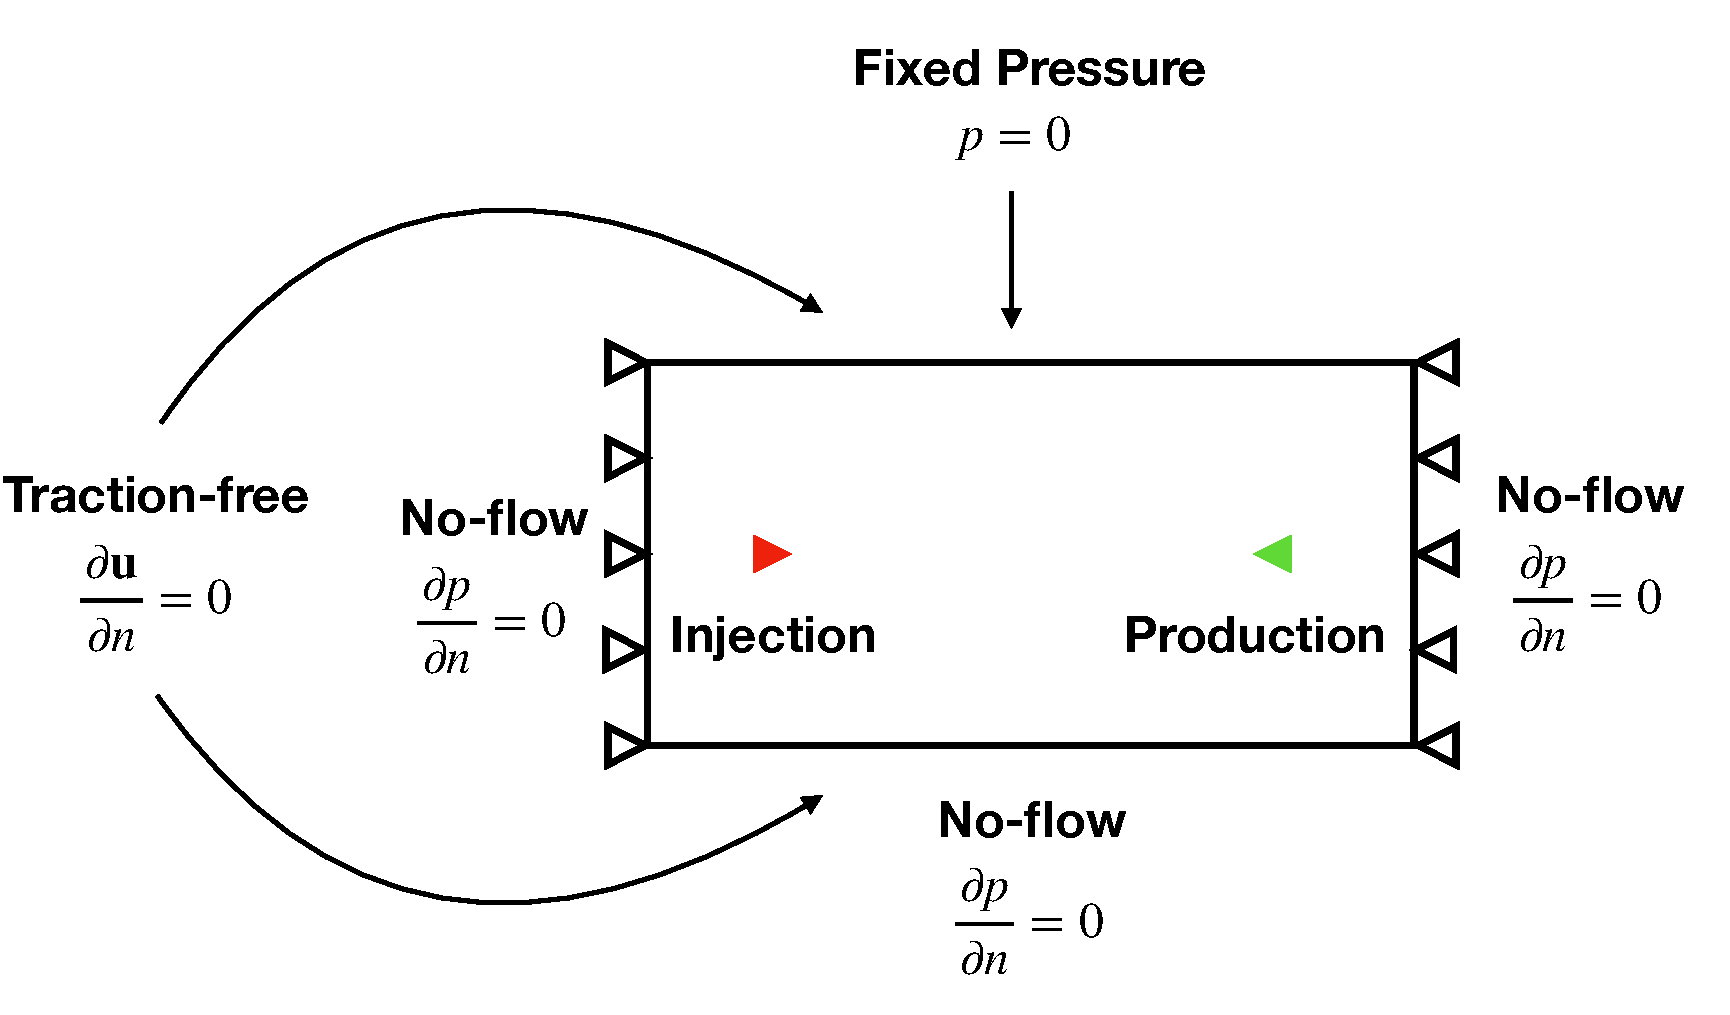
\includegraphics[width=0.5\textwidth]{../ip}~
  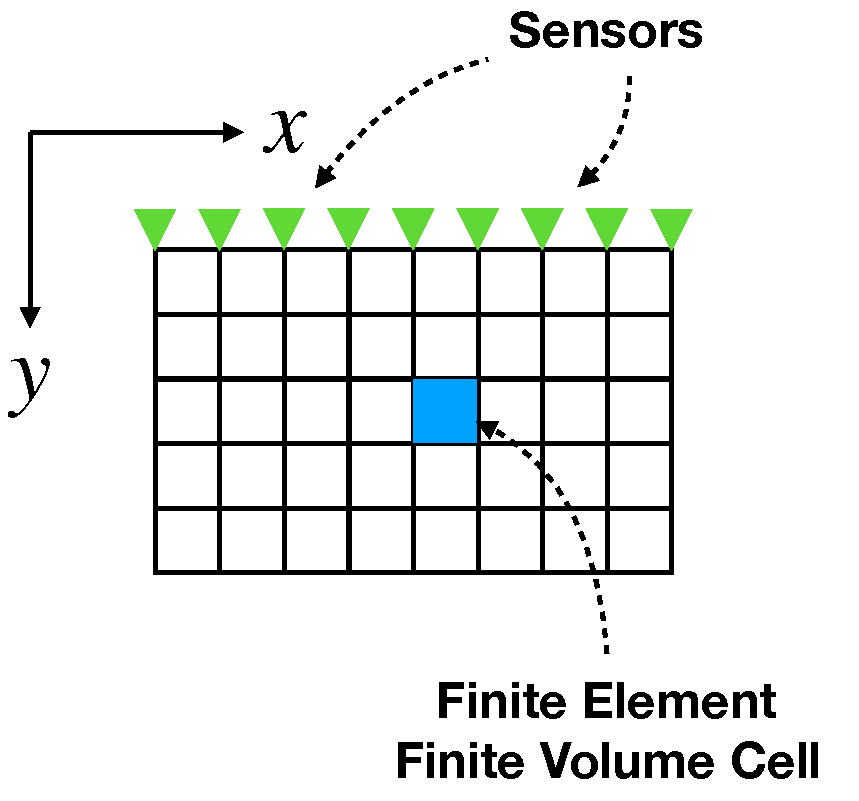
\includegraphics[width=0.3\textwidth]{../cell}
\end{figure}

\end{frame}


\begin{frame}
	\frametitle{Neural Networks: Inverse Modeling of Viscoelasticity}
	
	\begin{itemize}
		\item We propose the following form for modeling viscosity (assume the time step size is fixed):
		%   $$\bsigma^{n+1} = \mathcal{NN}_{\bt} (\bsigma^n, \bepsilon^n) + H\bepsilon^{n+1}$$
		$$\bsigma^{n+1} - \bsigma^{n} = \mathcal{NN}_{\bt} (\bsigma^n, \bepsilon^n) + H (\bepsilon^{n+1} - \bepsilon^n)$$
	\end{itemize}
	\begin{itemize}
		\item $H$ is a free optimizable \textcolor{red}{symmetric positive definite matrix} (SPD). Hence the numerical stiffness matrix is SPD.
		\item Implicit linear equation
		%   $$\bsigma^{n+1} = H(\bepsilon^{n+1} - \bepsilon^n) +  \left(\mathcal{NN}_{\bt} (\bsigma^n, \bepsilon^n)+H\bepsilon^n \right)$$
		$$\bsigma^{n+1} - H \bepsilon^{n+1} = - H \bepsilon^n
		+ \mathcal{NN}_{\bt} (\bsigma^n, \bepsilon^n) + \bsigma^{n}:= \mathcal{NN}_{\bt}^* (\bsigma^n, \bepsilon^n)$$
		\item Linear system to solve in each time step $\Rightarrow$ good balance between \textcolor{red}{numerical stability} and \textcolor{red}{computational cost}.
		\item Good performance in our numerical examples.
	\end{itemize}
\end{frame}

% \begin{frame}
% 	\frametitle{Neural Networks: Inverse Modeling of Viscoelasticity}
% 	\begin{figure}
% 		\centering
% 		\includegraphics[width=0.7\textwidth]{figures/strainstreess}
% 	\end{figure}
% \end{frame}

\begin{frame}
	\frametitle{Training Strategy and Numerical Stability}
	
	\begin{itemize}
		\item Physics constrained learning = improved numerical stability in predictive modeling.
		\item For simplicity, consider two strategies to train an NN-based constitutive relation using direct data $\{(\epsilon_o^n, \sigma_o^n)\}_n$
		$$\Delta \sigma^n = H \Delta \epsilon^n + \mathcal{NN}_{\bt} (\sigma^n, \epsilon^n),\quad H \succ 0$$
		\item Training with input-output pairs
		$$\min_{\bt} \sum_n \Big(\sigma_o^{n+1} - \big(H\epsilon_o^{n+1} +  \mathcal{NN}_{\bt}^* (\sigma_o^n, \epsilon_o^n)\big) \Big)^2$$
		\item Better stability using training on trajectory = \textcolor{red}{physics constrained learning}
		\begin{gather*}
		\min_{\bt} \ \sum_n (\sigma^n(\bt) - \sigma_o^n)^2 \\
		\text{s.t. }\text{I.C.} \ \sigma^1 = \sigma^1_o \text{ and time integrator\ }
		{\small \Delta \sigma^n = H \Delta \epsilon^n + \mathcal{NN}_{\bt} (\sigma^n, \epsilon^n)}
		\end{gather*}
	\end{itemize}
\end{frame}

\begin{frame}
	\frametitle{Experimental Data}
	
	\includegraphics[width=1.0\textwidth]{../experiment}
	
	{\scriptsize Experimental data from: Javidan, Mohammad Mahdi, and Jinkoo Kim. ``Experimental and numerical Sensitivity Assessment of Viscoelasticity for polymer composite Materials.'' Scientific Reports 10.1 (2020): 1--9.}
	
\end{frame}


\begin{frame}
	\frametitle{Inverse Modeling of Viscoelasticity}
	
	\begin{itemize}
		\item Comparison with space varying linear elasticity approximation
		\begin{equation*}
			\bsigma = H(x, y) \bepsilon
		\end{equation*}
	\end{itemize}
	\begin{figure}[hbt]
  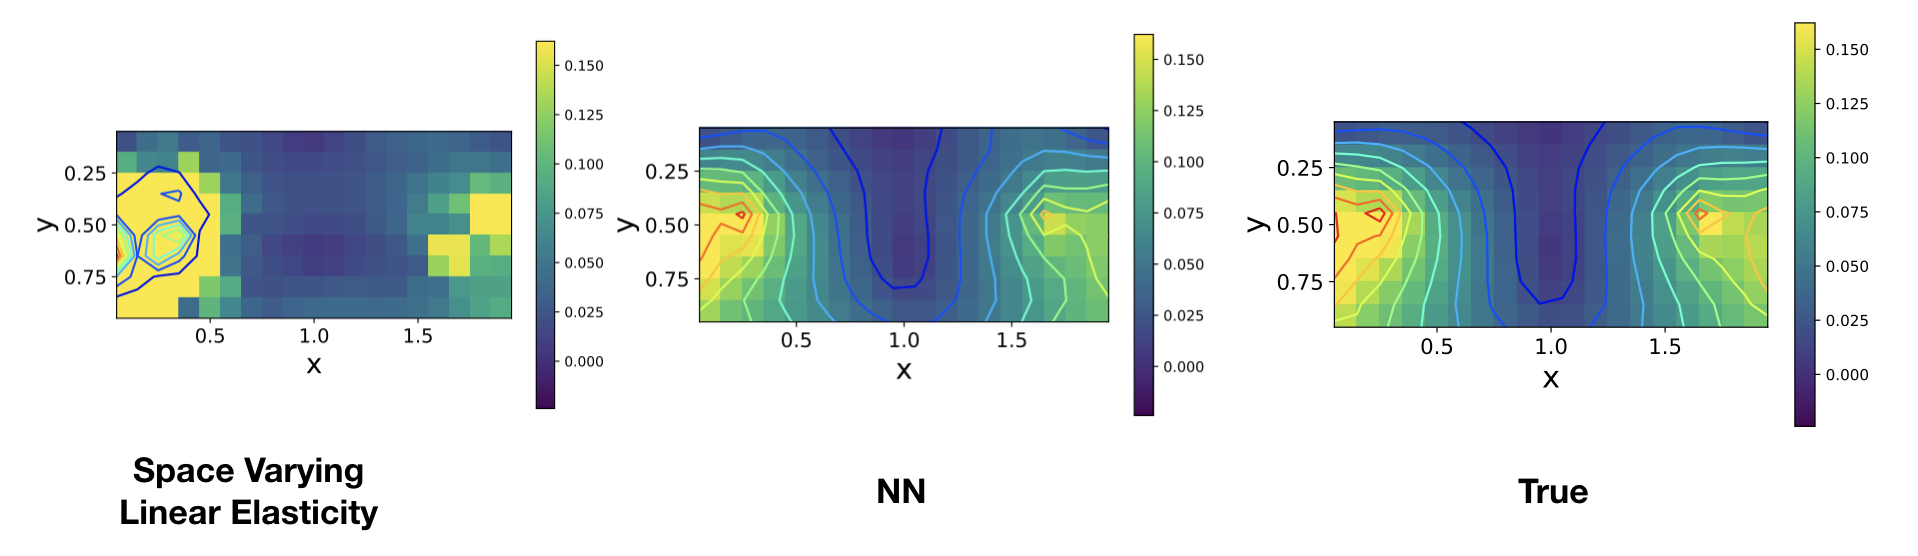
\includegraphics[width=1.0\textwidth]{../visco1}
\end{figure}

\end{frame}

\begin{frame}
	\frametitle{Inverse Modeling of Viscoelasticity}
	\begin{figure}[hbt]
  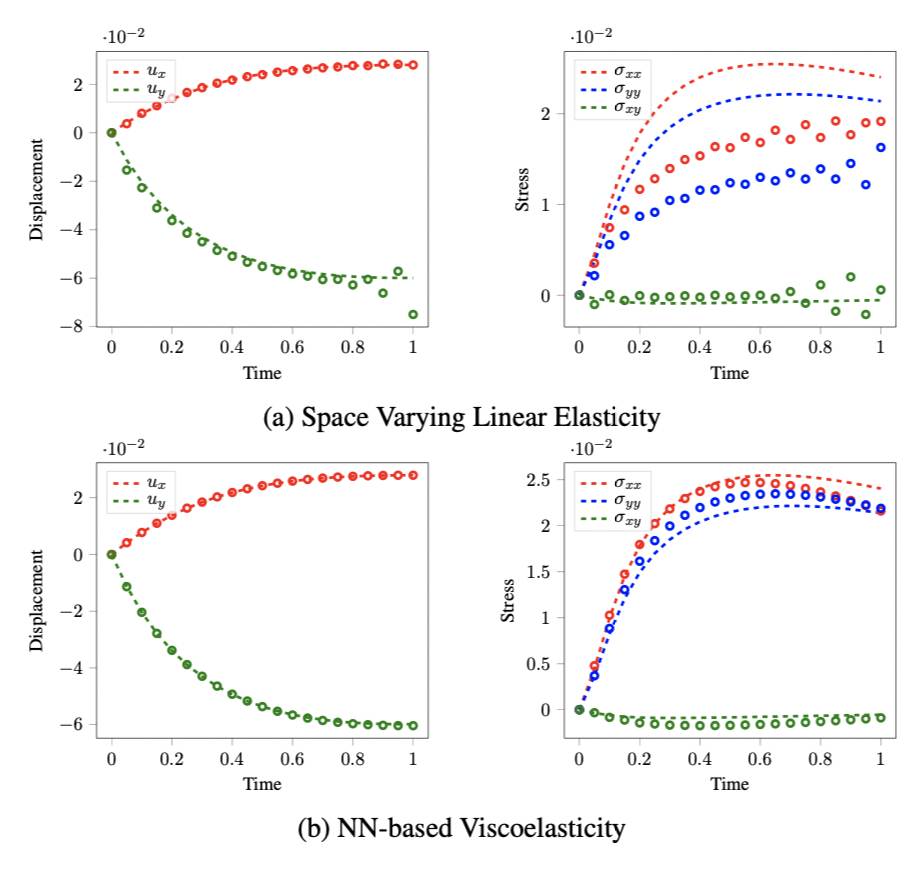
\includegraphics[width=0.7\textwidth]{../visco2}
\end{figure}

\end{frame}


\section{ADCME: Scientific Machine Learning for Inverse Modeling}

\begin{frame}
	\frametitle{Physical Simulation as a Computational Graph}
	\begin{figure}[hbt]
		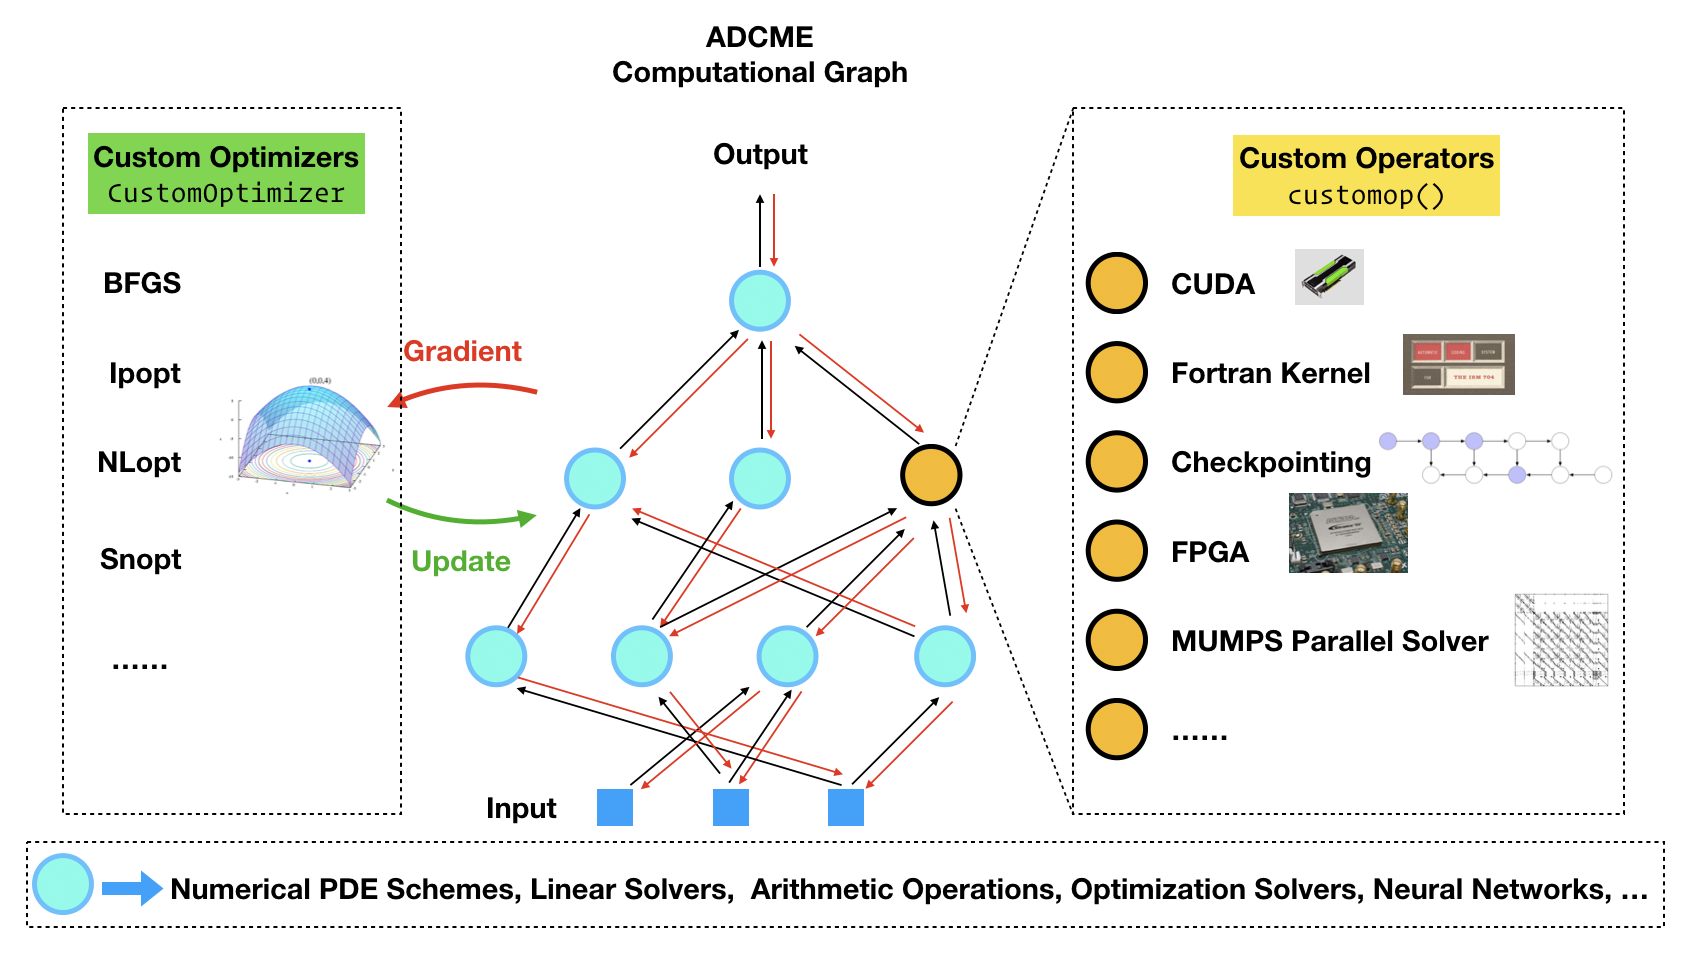
\includegraphics[width=1.0\textwidth]{../custom.png}
	\end{figure}
\end{frame}

\begin{frame}
	\frametitle{A General Approach to Inverse Modeling}
	\begin{figure}[hbt]
  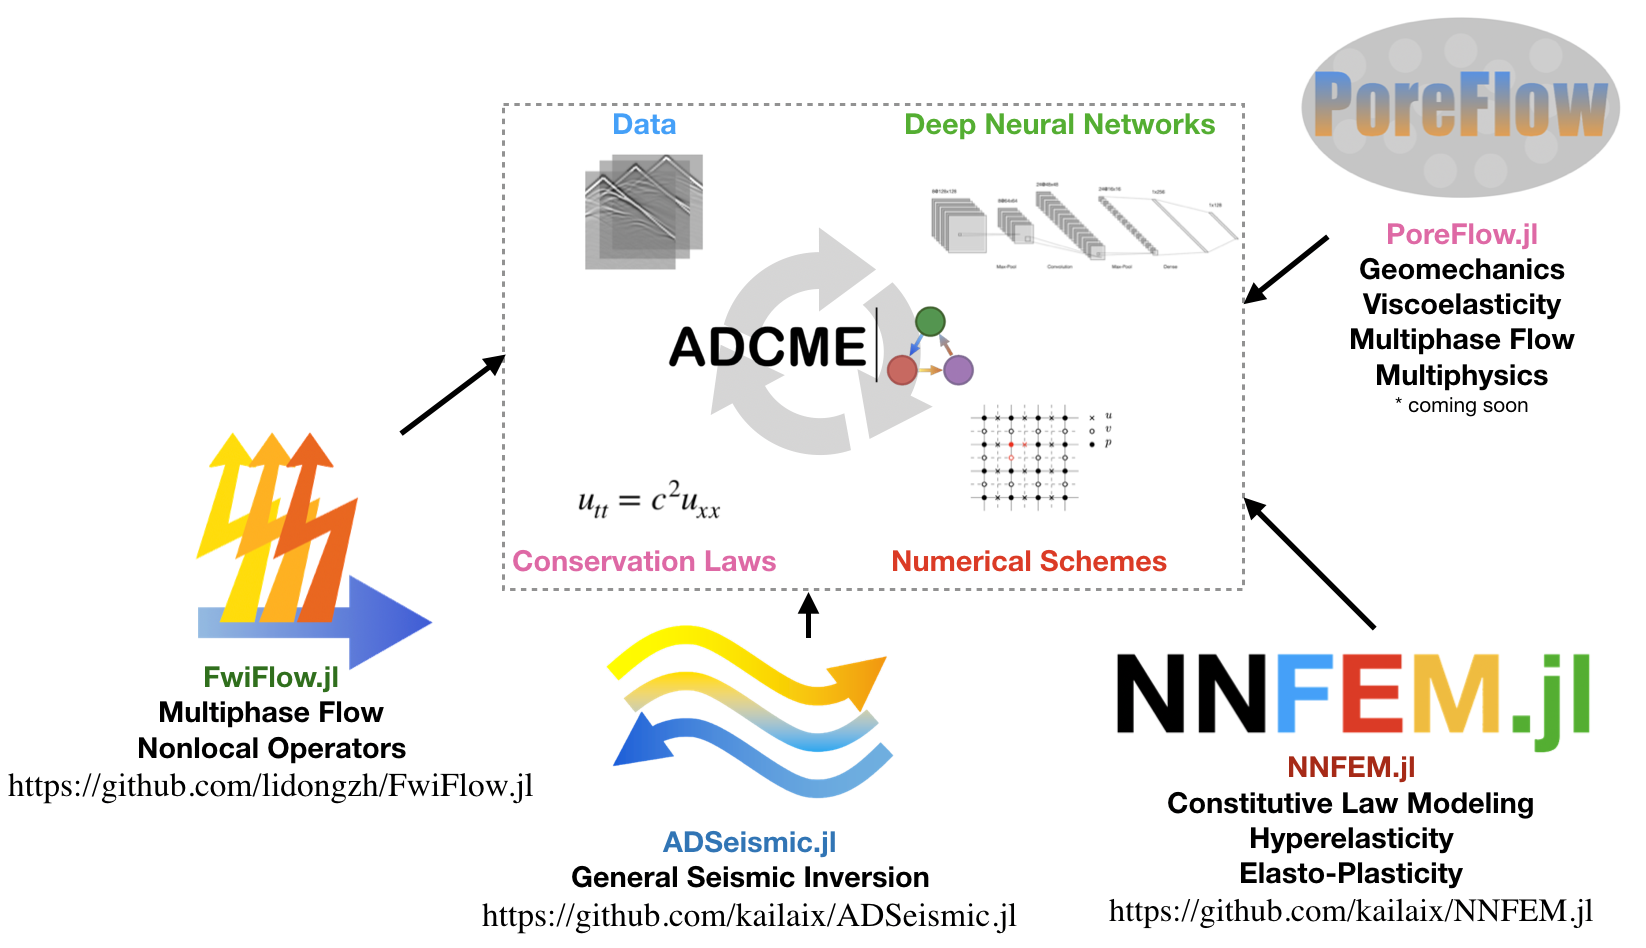
\includegraphics[width=1.0\textwidth]{../summary.png}
\end{figure}
%
\end{frame}

%}
%\usebackgroundtemplate{}
%----------------------------------------------------------------------------------------
%    PRESENTATION SLIDES
%----------------------------------------------------------------------------------------

%------------------------------------------------



\end{document} 